\documentclass[11pt]{article}

\usepackage[utf8]{inputenc}
\usepackage[T1]{fontenc}
\usepackage{multicol}
\usepackage{amsthm}
\usepackage{amsmath}
\usepackage{amssymb}
\usepackage{mathtools}
\usepackage{dsfont}
\usepackage{bm}
\usepackage{bbm}
\usepackage{xparse}
\usepackage{physics}
\usepackage{empheq}
\usepackage{url}
\usepackage{hyperref}
\usepackage[affil-it]{authblk}
\usepackage{tikz}
\usetikzlibrary{quotes,angles,calc}
\usepackage{rotating}
\usepackage{graphicx}
\usepackage[linesnumbered,ruled,vlined]{algorithm2e}

\usepackage{pgfplots}
\pgfplotsset{compat = newest}

\usepackage[top=3cm,bottom=2cm,right=2cm,left=2cm]{geometry}

\theoremstyle{definition}
\newtheorem{theo}{Theorem}[section]
\newtheorem{lem}[theo]{Lemma}
\newtheorem{cor}[theo]{Corollary}
\newtheorem{prop}[theo]{Proposition}
\newtheorem{defi}[theo]{Definition}
\newtheorem{conj}[theo]{Conjecture}

\newtheorem{theo*}{Theorem}

\theoremstyle{remark}
\newtheorem*{rk}{Remark}

\DeclareMathOperator{\Poi}{\text{Poi}}
\DeclareMathOperator{\Ber}{\text{Ber}}
\DeclareMathOperator{\Bin}{\text{Bin}}
\DeclareMathOperator{\maxi}{\text{maximize}}
\DeclareMathOperator{\mini}{\text{minimize}}
\DeclareMathOperator{\st}{\text{subject to}}
\DeclarePairedDelimiter\ceil{\lceil}{\rceil}
\DeclarePairedDelimiter\floor{\lfloor}{\rfloor}
\DeclarePairedDelimiterX\set[1]\lbrace\rbrace{\def\given{\;\delimsize\vert\;}#1}

\newcommand{\OF}[1]{\textcolor{blue}{OF: #1}}

\title{\bfseries Broadcast Channels with Non-Signaling Correlations}
\author{Omar Fawzi\footnote{Univ Lyon, ENS Lyon, UCBL, CNRS, Inria,  LIP, F-69342, Lyon Cedex 07, France. \href{mailto:omar.fawzi@ens-lyon.fr}{\texttt{omar.fawzi@ens-lyon.fr}}} \qquad Paul Fermé\footnote{Univ Lyon, ENS Lyon, UCBL, CNRS, Inria, LIP, F-69342, Lyon Cedex 07, France. \href{mailto:paul.ferme@ens-lyon.fr}{\texttt{paul.ferme@ens-lyon.fr}}}
}
\date{}

\begin{document}
\maketitle

\section{Introduction}
TODO

\section{Broadcast Channels}
\subsection{Classical Quantities}
Formally, a broadcast channel is given by a conditional probability distributions on input $\mathcal{X}$ and two outputs $\mathcal{Y}_1$ and $\mathcal{Y}_2$, so $W := \left(W(y_1,y_2|x)\right)_{y_1 \in \mathcal{Y}_1, y_2 \in \mathcal{Y}_2, x \in \mathcal{X}}$, where $W(y_1y_2|x) \geq 0, \sum_{y_1 \in \mathcal{Y}_1, y_2 \in \mathcal{Y}_2} W_b(y_b|x) = 1$. We define its marginal $W_1$ and $W_2$ by $W_1(y_1|x) := \sum_{y_2 \in \mathcal{Y}_2} W(y_1y_2|x)$ and $W_2(y_2|x) := \sum_{y_1 \in \mathcal{Y}_1} W(y_1y_2|x)$. We will denote such a broadcast channel by $W : \mathcal{X} \rightarrow \mathcal{Y}_1 \times \mathcal{Y}_2$.

\subsubsection{$\mathrm{S}_{\text{average}}(W,k_1,k_2)$}
For a broadcast channel $W : \mathcal{X} \rightarrow \mathcal{Y}_1 \times \mathcal{Y}_2$, several measures of merits can be considered. We will focus first on the maximal average of the probability of sending $k_1k_2$ messages and decoding correctly the $k_1$ messages of receiver $1$ with the probability of decoding correctly the $k_2$ messages of receiver $2$, which we will denote by $\mathrm{S}_{\text{average}}(W,k_1,k_2)$. This means that one can encode $k_1k_2$ messages in $\mathcal{X}$ through $e$, and then decode $k_1$ messages from the output in $\mathcal{Y}_1$ with $d_1$ for receiver $1$ and $k_2$ messages from the output in $\mathcal{Y}_2$ with $d_2$ for receiver $2$. This leads to the following optimization program for $\mathrm{S}_{\text{average}}(W,k_1,k_2)$:
\begin{equation}
  \begin{aligned}
    \mathrm{S}_{\text{average}}(W,k_1,k_2) := &&\underset{e,d_1,d_2}{\maxi} &&& \frac{1}{k_1k_2}\sum_{x,y_1,y_2,i_1,i_2} W(y_1y_2|x)e(x|i_1i_2)\frac{d_1(i_1|y_1) + d_2(i_2|y_2)}{2}\\
    &&\st &&& \sum_{x \in \mathcal{X}} e(x|i_1i_2) = 1, \forall i_1 \in [k_1], i_2 \in [k_2]\\
    &&&&& \sum_{i_1 \in [k_1]} d_1(y_1|i_1) = 1, \forall y_1 \in \mathcal{Y}_1\\
    &&&&& \sum_{i_2 \in [k_2]} d_2(y_2|i_2) = 1, \forall y_2 \in \mathcal{Y}_2\\
    &&&&& e(x|i_1i_2), d_1(y_1|i_1), d_2(y_2|i_2) \geq 0
  \end{aligned}
\end{equation}

First, one can rewrite this linear program in a more convenient way, proving that this $\mathrm{S}_{\text{average}}(W,k_1,k_2)$ depends only on the marginals of $W$:
\begin{prop}
  \begin{equation}
  \begin{aligned}
    \mathrm{S}_{\text{average}}(W,k_1,k_2) = &&\underset{e,d_1,d_2}{\maxi} &&& \frac{1}{2k_1k_2}\sum_{x,y_1,i_1} W_1(y_1|x)d_1(i_1|y_1)\sum_{i_2} e(x|i_1i_2)\\
    &&+&&& \frac{1}{2k_1k_2}\sum_{x,y_2,i_2} W_2(y_2|x)d_2(i_2|y_2)\sum_{i_1} e(x|i_1i_2)\\
    &&\st &&& \sum_{x \in \mathcal{X}} e(x|i_1i_2) = 1, \forall i_1 \in [k_1], i_2 \in [k_2]\\
    &&&&& \sum_{i \in [k_1]} d_1(y_1|i_1) = 1, \forall y_1 \in \mathcal{Y}_1\\
    &&&&& \sum_{i \in [k_2]} d_2(y_2|i_2) = 1, \forall y_2 \in \mathcal{Y}_2\\
    &&&&& e(x|i_1i_2), d_1(y_1|i_1), d_2(y_2|i_2) \geq 0
  \end{aligned}
\end{equation}

\end{prop}


As a linear program is optimized in its extremal points \cite{TODO}, $\mathrm{S}_{\text{average}}(W,k_1,k_2)$ is alternatively given by the following combinatorial optimization problem:

\begin{prop}
  \[ \mathrm{S}_{\text{average}}(W,k_1,k_2) = \underset{C : [k_1] \times [k_2] \rightarrow \mathcal{X}}{\maxi} \ \frac{1}{2k_1k_2} \left(\underbrace{\sum_{y_1 \in \mathcal{Y}_1} \max_{i_1 \in [k_1]}\sum_{i_2 \in [k_2]} W_1(y_1|C(i_1,i_2))}_{=: f_W^1(C,k_1,k_2)} + \underbrace{\sum_{y_2 \in \mathcal{Y}_2} \max_{i_2 \in [k_2]} \sum_{i_1 \in [k_1]} W_2(y_2|C(i_1,i_2))}_{=: f_W^2(C,k_1,k_2)}\right) \ . \]
\end{prop}
\begin{proof}
  Idea: $C(i_1,i_2)=x$ s.t. $e(x|i_1i_2)=1$ (exists uniquely). Then:
  \[ \sum_{x,y_1,i_1} W_1(y_1|x)d_1(i_1|y_1)\sum_{i_2} e(x|i_1i_2) = \sum_{y_1,i_1}d_1(i_1|y_1) \sum_{i_2} W_1(y_1|C(i_1,i_2)) \ .\]
  So the $d_1$ that maximizes this value gives the value from proposition.
\end{proof}

Since broadcast channels are more general than one-way channels (by defining $W_1(y_1|x):=\hat{W}(y_1|x)$ for $\hat{W}$ a one-way channel and taking $W_2(y_2|x)=\frac{1}{|\mathcal{Y}_2|}$ a completely trivial channel), computing a single value $\mathrm{S}_{\text{average}}(W,k_1,k_2)$ is \textrm{NP}-hard, and it is even \textrm{NP}-hard to approximate $\mathrm{S}_{\text{average}}(W,k_1,k_2)$ within a better ratio than $\left(1-e^{-1}\right)$, as a consequence of the hardness result on $\mathrm{S}_{\text{average}}(W,k)$ shown in \cite{BF18}.

\subsubsection{$\mathrm{S}(W,k_1,k_2)$}
We will now focus on the probability of sending $k_1k_2$ messages and decoding correctly the $k_1$ messages of receiver $1$ and decoding correctly the $k_2$ messages of receiver $2$ at the same time, which we will denote by $\mathrm{S}(W,k_1,k_2)$. This means that one can encode $k_1k_2$ messages in $\mathcal{X}$ through $e$, and then decode $k_1$ messages from the output in $\mathcal{Y}_1$ with $d_1$ for receiver $1$ and $k_2$ messages from the output in $\mathcal{Y}_2$ with $d_2$ for receiver $2$. This leads to the following optimization program for $\mathrm{S}(W,k_1,k_2)$:
\begin{equation}
  \begin{aligned}
    \mathrm{S}(W,k_1,k_2) := &&\underset{e,d_1,d_2}{\maxi} &&& \frac{1}{k_1k_2}\sum_{x,y_1,y_2,i_1,i_2} W(y_1y_2|x)e(x|i_1i_2)d_1(i_1|y_1)d_2(i_2|y_2)\\
    &&\st &&& \sum_{x \in \mathcal{X}} e(x|i_1i_2) = 1, \forall i_1 \in [k_1], i_2 \in [k_2]\\
    &&&&& \sum_{i_1 \in [k_1]} d_1(y_1|i_1) = 1, \forall y_1 \in \mathcal{Y}_1\\
    &&&&& \sum_{i_2 \in [k_2]} d_2(y_2|i_2) = 1, \forall y_2 \in \mathcal{Y}_2\\
    &&&&& e(x|i_1i_2), d_1(y_1|i_1), d_2(y_2|i_2) \geq 0
  \end{aligned}
\end{equation}

However, $\mathrm{S}(W,k_1,k_2)$ and $\mathrm{S}_{\text{average}}(W,k_1,k_2)$ define the same capacity regions. Indeed, let us focus on the error probabilities than the success ones. Call them respectively $\mathcal{E}(W,k_1,k_2) := 1-\mathrm{S}(W,k_1,k_2)$ and $\mathcal{E}_{\text{average}}(W,k_1,k_2) := 1-\mathrm{S}_{\text{average}}(W,k_1,k_2)$. We have, given an optimal solution $(e,d_1,d_2)$ for $S$:

\begin{equation}
  \begin{aligned}
    \mathcal{E}(W,k_1,k_2) &= 1 -  \frac{1}{k_1k_2}\left(\sum_{x,y_1,y_2,i_1,i_2} W(y_1y_2|x)e(x|i_1i_2)d_1(i_1|y_1)d_2(i_2|y_2)\right)\\
    &=\frac{1}{k_1k_2}\left(k_1k_2-\sum_{x,y_1,y_2,i_1,i_2} W(y_1y_2|x)e(x|i_1i_2)d_1(i_1|y_1)d_2(i_2|y_2)\right)\\
    &=\frac{1}{k_1k_2}\left(\sum_{x,i_1,i_2} e(x|i_1i_2)-\sum_{x,y_1,y_2,i_1,i_2} W(y_1y_2|x)e(x|i_1i_2)d_1(i_1|y_1)d_2(i_2|y_2)\right)\\
    &=\frac{1}{k_1k_2}\left(\sum_{x,y_1,y_2,i_1,i_2} W(y_1y_2|x)e(x|i_1i_2)-\sum_{x,y_1,y_2,i_1,i_2} W(y_1y_2|x)e(x|i_1i_2)d_1(i_1|y_1)d_2(i_2|y_2)\right)\\
    &=\frac{1}{k_1k_2}\left(\sum_{x,y_1,y_2,i_1,i_2} W(y_1y_2)e(x|i_1i_2)\left[1-d_1(i_1|y_1)d_2(i_2|y_2)\right]\right) \ .\\
  \end{aligned}
\end{equation}

Similarly, we have that $\mathcal{E}_{\text{average}}(W,k_1,k_2)=\frac{1}{k_1k_2}\left(\sum_{x,y_1,y_2,i_1,i_2} W(y_1y_2)e(x|i_1i_2)\left[1-\frac{d_1(i_1|y_1)+d_2(i_2|y_2)}{2}\right]\right) = \frac{1}{k_1k_2}\left(\sum_{x,y_1,y_2,i_1,i_2} W(y_1y_2)e(x|i_1i_2)\left[\frac{1-d_1(i_1|y_1)}{2} + \frac{1-d_2(i_2|y_2)}{2}\right]\right)$ if $(e,d_1,d_2)$ is an optimal solution for $S_{\text{average}}$.

However, given any decoding scheme $d_1,d_2$ we have that:
\[1-d_1(i_1|y_1)d_2(i_2|y_2) \geq \max\left(1-d_1(i_1|y_1),1-d_2(i_2|y_2)\right) \geq 1-\frac{d_1(i_1|y_1)+d_2(i_2|y_2)}{2} \ , \]
and:
\[1-d_1(i_1|y_1)d_2(i_2|y_2) \leq (1-d_1(i_1|y_1)) + (1-d_2(i_2|y_2)) \ . \]

This means that $\mathcal{E}_{\text{average}}(W,k_1,k_2) \leq \mathcal{E}(W,k_1,k_2) \leq 2\mathcal{E}_{\text{average}}(W,k_1,k_2)$. Thus, up to a constant $2$, a solution for both quantities gives the same error. In particular, this implies that the capacity regions are the same.


\subsection{Non-Signaling Assistance}
\subsubsection{Non-Signaling Assistance Between the Decoders}
We will show in that section that allowing some non-signaling assistance between the decoders do not increase the capacity regions in both the exact and average scenarios.

First, when non-signaling assistance between the decoders is given to a broadcast channel, both decoders $d_1,d_2$ are replaced by a non-signaling box $d(j_1j_2|y_1y_2)$ replacing the product $d_1(j_1|y_1)d_2(j_2|y_2)$. However, in the average scenario, since the objective function does not depend on the product $d_1(j_1|y_1)d_2(j_2|y_2)$ but only on the marginals $d_1(j_1|y_1)$ and $d_2(j_2|y_2)$, the non-signaling box won't give additional decoding power. Indeed, we have that:
\begin{equation}
  \begin{aligned}
    \mathrm{S}_{\text{average}}^{\mathrm{NS}_{d_1d_2}}(W,k_1,k_2) &= \frac{1}{2k_1k_2}\sum_{x,y_1,i_1} W_1(y_1|x)\left(\sum_{j_2}d(i_1j_2|y_1y_2)\right)\sum_{i_2} e(x|i_1i_2)\\
    &+ \frac{1}{2k_1k_2} \sum_{x,y_2,i_2} W_2(y_2|x)\left(\sum_{j_1}d(j_1i_2|y_1y_2)\right)\sum_{i_1} e(x|i_1i_2) \ .
  \end{aligned}
\end{equation}

Thus, by defining $d_1(j_1|y_1) := \sum_{j_2}d(j_1j_2|y_1y_2)$ and $d_2(j_2|y_2) := \sum_{j_1}d(j_1j_2|y_1y_2)$, which are well-defined since $d$ is non-signaling, one recovers a solution of $\mathrm{S}_{\text{average}}(W,k_1,k_2)$ with the same value as $\mathrm{S}_{\text{average}}^{\mathrm{NS}_{d_1d_2}}(W,k_1,k_2)$. Since the inequality is obvious in the other direction, we have that $\mathrm{S}_{\text{average}}(W,k_1,k_2)=\mathrm{S}_{\text{average}}^{\mathrm{NS}_{d_1d_2}}(W,k_1,k_2)$.

On the other hand, in the exact case, the non-signaling bow between the decoders leads to the following value:
\[ \mathrm{S}^{\mathrm{NS}_{d_1d_2}}(W,k_1,k_2) = \frac{1}{k_1k_2}\sum_{x,y_1,y_2,i_1,i_2} W(y_1y_2|x)e(x|i_1i_2)d(i_1i_2|y_1y_2) \ . \]

This should be compared to the average case:
\[ \mathrm{S}_{\text{average}}^{\mathrm{NS}_{d_1d_2}}(W,k_1,k_2) = \frac{1}{k_1k_2}\sum_{x,y_1,y_2,i_1,i_2} W(y_1y_2|x)e(x|i_1i_2)\left[\frac{\sum_{j_2}d(i_1j_2|y_1y_2)+\sum_{j_1}d(j_1i_2|y_1y_2)}{2}\right] \ . \]

Similarly to what was done classicaly, we focus on the error probabilities rather than success probabilities. This leads again to:

\[ \mathcal{E}^{\mathrm{NS}_{d_1d_2}}(W,k_1,k_2) = \frac{1}{k_1k_2}\sum_{x,y_1,y_2,i_1,i_2} W(y_1y_2|x)e(x|i_1i_2)\left[1-d(i_1i_2|y_1y_2)\right] \ , \]
and:
\[ \mathcal{E}_{\text{average}}^{\mathrm{NS}_{d_1d_2}}(W,k_1,k_2) = \frac{1}{k_1k_2}\sum_{x,y_1,y_2,i_1,i_2} W(y_1y_2|x)e(x|i_1i_2)\left[\frac{1-\sum_{j_2}d(i_1j_2|y_1y_2)}{2}+\frac{1-\sum_{j_1}d(j_1i_2|y_1y_2)}{2}\right] \ . \]

But we have that:

\[ 1-d(i_1i_2|y_1y_2) \geq \max\left(1-\sum_{j_2}d(i_1j_2|y_1y_2),1-\sum_{j_1}d(j_1i_2|y_1y_2)\right) \geq \frac{1-\sum_{j_2}d(i_1j_2|y_1y_2)}{2}+\frac{1-\sum_{j_1}d(j_1i_2|y_1y_2)}{2} \ ,\]

since $d(j_1j_2|y_1y_2) \geq 0$, and we have that:
\[ 1-\sum_{j_2}d(i_1j_2|y_1y_2)+1-\sum_{j_1}d(j_1i_2|y_1y_2) = 1-d(i_1i_2|y_1y_2) + 1-\sum_{j_2\not=i_2}d(i_1j_2|y_1y_2)-\sum_{j_1\not=i_1}d(j_1i_2|y_1y_2) \geq 1-d(i_1i_2|y_1y_2) \ ,\]
since $\sum_{(j_1,j_2) \in S} d(j_1j_2|y_1y_2) \leq 1$ for $S$ a subset of $[k_1] \times [k_2]$.

Thus, this implies that  $\mathcal{E}_{\text{average}}^{\mathrm{NS}_{d_1d_2}}(W,k_1,k_2) \leq \mathcal{E}^{\mathrm{NS}_{d_1d_2}}(W,k_1,k_2) \leq 2\mathcal{E}_{\text{average}}^{\mathrm{NS}_{d_1d_2}}(W,k_1,k_2)$. Thus, up to a constant $2$, a solution for both quantities gives the same error. In particular, this implies that the capacity regions are the same.

Furhtermore, since $\mathcal{E}_{\text{average}}^{\mathrm{NS}_{d_1d_2}}(W,k_1,k_2)=\mathcal{E}_{\text{average}}(W,k_1,k_2)$, we have that up to a constant $4$, $\mathcal{E}^{\mathrm{NS}_{d_1d_2}}(W,k_1,k_2)$ is the same as $ \mathcal{E}(W,k_1,k_2)$. Thus the capacity regions of these four quantities are the same. We conclude that non-signaling assistance between the decoders is useless for broadcast channels.

\subsubsection{Non-Signaling Assistance Between the Encoder and one Decoder}
When non-signaling assistance between the encoder and the first decoder is given to a broadcast channel, the product of the encoder $e$ and the first decoder $d_1$ is replaced by a non-signaling box $P(xj_1|(i_1i_2)y_1)$. This leads to the following optimization program in the exact case:

\begin{equation}
  \begin{aligned}
    \mathrm{S}^{\mathrm{NS}_{e,d_1}}(W,k_1,k_2) := &&\underset{P,d_2}{\maxi} &&& \frac{1}{k_1k_2}\sum_{x,y_1,y_2,i_1,i_2} W(y_1y_2|x)P(xi_1|(i_1i_2)y_1)d(i_2|y_2)\\
    &&\st &&& \sum_{x,j_1} P(xj_1|(i_1i_2)y_1) = 1\\
    &&&&& \sum_x P(xj_1|(i_1i_2)y_1) = \sum_x P(xj_1|(i_1'i_2')y_1)\\
    &&&&& \sum_{j_1} P(xj_1|(i_1i_2)y_1) = \sum_{j_1} P(xj_1|(i_1i_2)y_1')\\
    &&&&& \sum_{i_2} d(y_2|i_2) = 1\\
    &&&&& P(xj_1|i_1i_2), d(y_2|i_2) \geq 0
  \end{aligned}
\end{equation}

An equivalent, more convenient and smaller program computing $\mathrm{S}^{\mathrm{NS}_{e,d_1}}(W,k_1,k_2)$ can be found:

\begin{prop}
\begin{equation}
  \begin{aligned}
    \mathrm{S}^{\mathrm{NS}_{e,d_1}}(W,k_1,k_2) = &&\underset{p,r,r^1,r^2}{\maxi} &&& \frac{1}{k_1k_2}\sum_{x,y_1,y_2} W(y_1y_2|x)\sum_{i_2}d(i_2|y_2)r^{i_2}_{x,y_1}\\
    &&\st &&& \sum_{x} r^{i_2}_{x,y_1} = 1\\
    &&&&& \sum_{x} p^{i_2}_x = k_1\\
    &&&&& 0 \leq r^{i_2}_{x,y_1} \leq p^{i_2}_x\\
    &&&&& \sum_{i_2} d(y_2|i_2) = 1\\
    &&&&& d(y_2|i_2) \geq 0
  \end{aligned}
\end{equation}
\end{prop}

\begin{proof}
  One can checks that given a solution of the original program, the following choice of variables is a valid solution of the second program achieving the same objective value:
\begin{equation}
  \begin{aligned}
    &r^{i_2}_{x,y_1} := \sum_{i_1} P(xi_1|(i_1i_2)y_1)\ ,\\
    &p^{i_2}_x := \sum_{j_1,i_1} P(xj_1|(i_1i_2)y_1) \ .\\
  \end{aligned}
\end{equation}

For the other direction, given those variables, a non-signaling probability distribution $P(xj_1|(i_1i_2)y_1)$ is given by, for $j_1 \not= i_1$:
\begin{equation}
  \begin{aligned}
    &P(xi_1|(i_1i_2)y_1) = \frac{r^{i_2}_{x,y_1}}{k_1}  \ ,\\
    &P(xj_1|(i_1i_2)y_1) = \frac{p^{i_2}_x - r^{i_2}_{x,y_1}}{k_1(k_1-1)}  \ .\\
  \end{aligned}
\end{equation}
\end{proof}

\subsubsection{Full Non-Signaling Assistance}
When full non-signaling assistance is given between the three parties of a broadcast channel, both decoders $d_1,d_2$ and the encoder $e$ are replaced by a non-signaling box $P(xj_1j_2|(i_1i_2)y_1y_2)$. Then, the maximal average of the probability of sending $k_1k_2$ messages and decoding correctly the $k_1$ messages of receiver $1$ with the probability of decoding correctly the $k_2$ messages of receiver $2$ with non signaling assistance, which we call $\mathrm{S}_{\text{average}}^{\mathrm{NS}}(W,k_1,k_2)$, is given by the following linear program, where the constraints translate the fact that $P$ is a non-signaling box:

\begin{equation}
  \begin{aligned}
    \mathrm{S}_{\text{average}}^{\mathrm{NS}}(W,k_1,k_2) := &&\underset{P}{\maxi} &&& \frac{1}{2k_1k_2}\sum_{x,y_1,i_1} W_1(y_1|x)\sum_{j_2,i_2} P(xi_1j_2|(i_1i_2)y_1y_2)\\
    &&+&&& \frac{1}{2k_1k_2}\sum_{x,y_2,i_2} W_2(y_2|x) \sum_{j_1,i_1} P(xj_1i_2|(i_1i_2)y_1y_2)\\
    &&\st &&& \sum_{x \in \mathcal{X}} P(xj_1j_2|(i_1i_2)y_1y_2) = \sum_{x \in \mathcal{X}} P(xj_1j_2|(i_1'i_2')y_1y_2)\\
    &&&&& \sum_{j_1 \in [k_1]} P(xj_1j_2|(i_1i_2)y_1y_2) = \sum_{j_1 \in [k_1]} P(xj_1j_2|(i_1i_2)y_1'y_2)\\
    &&&&& \sum_{j_2 \in [k_2]} P(xj_1j_2|(i_1i_2)y_1y_2) = \sum_{j_2 \in [k_2]} P(xj_1j_2|(i_1i_2)y_1y_2')\\
    &&&&& \sum_{x \in \mathcal{X}, j_1 \in [k_1], j_2 \in [k_2]} P(xj_1j_2|(i_1i_2)y_1y_2) = 1\\
    &&&&& P(xj_1j_2|(i_1i_2)y_1y_2) \geq 0
  \end{aligned}
\end{equation}

Since it is given as a linear program, the complexity of computing $\mathrm{S}_{\text{average}}^{\mathrm{NS}}(W)$ is polynomial in the number of variables and constraints, which is a polynomial in $|\mathcal{X}|,|\mathcal{Y}_1|,|\mathcal{Y}_2|$ and $k$. Also, as it is easy to check that a classical strategy is a particular case of a non-signaling assisted strategy, we have that $\mathrm{S}_{\text{average}}^{\mathrm{NS}}(W,k_1,k_2) \geq \mathrm{S}_{\text{average}}(W,k_1,k_2)$.

Similarly for the exact case:
\begin{equation}
  \begin{aligned}
    \mathrm{S}^{\mathrm{NS}}(W,k_1,k_2) := &&\underset{P}{\maxi} &&& \frac{1}{k_1k_2}\sum_{x,y_1,y_2,i_1,i_2} W_1(y_1y_2|x)P(xi_1i_2|(i_1i_2)y_1y_2)\\
    &&\st &&& \sum_{x \in \mathcal{X}} P(xj_1j_2|(i_1i_2)y_1y_2) = \sum_{x \in \mathcal{X}} P(xj_1j_2|(i_1'i_2')y_1y_2)\\
    &&&&& \sum_{j_1 \in [k_1]} P(xj_1j_2|(i_1i_2)y_1y_2) = \sum_{j_1 \in [k_1]} P(xj_1j_2|(i_1i_2)y_1'y_2)\\
    &&&&& \sum_{j_2 \in [k_2]} P(xj_1j_2|(i_1i_2)y_1y_2) = \sum_{j_2 \in [k_2]} P(xj_1j_2|(i_1i_2)y_1y_2')\\
    &&&&& \sum_{x \in \mathcal{X}, j_1 \in [k_1], j_2 \in [k_2]} P(xj_1j_2|(i_1i_2)y_1y_2) = 1\\
    &&&&& P(xj_1j_2|(i_1i_2)y_1y_2) \geq 0
  \end{aligned}
\end{equation}

Equivalent, more convenient and smaller linear programs computing $\mathrm{S}_{\text{average}}^{\mathrm{NS}}(W,k_1,k_2)$ and $\mathrm{S}^{\mathrm{NS}}(W,k_1,k_2)$ can be found:

\begin{prop}
\begin{equation}
  \begin{aligned}
    \mathrm{S}_{\text{average}}^{\mathrm{NS}}(W,k_1,k_2) = &&\underset{p,r,r^1,r^2}{\maxi} &&& \frac{1}{2k_1k_2}\left(\sum_{x,y_1} W_1(y_1|x)r^1_{x,y_1} + \sum_{x,y_2} W_2(y_2|x)r^2_{x,y_2}\right)\\
    &&\st &&& \sum_{x} r_{x,y_1,y_2} = 1\\
    &&&&&\sum_{x} r^1_{x,y_1} = k_2\\
    &&&&& \sum_{x} r^2_{x,y_2} = k_1\\
    &&&&& \sum_{x} p_x = k_1k_2\\
    &&&&& 0 \leq r_{x,y_1,y_2} \leq r^1_{x,y_1}, r^2_{x,y_2} \leq p_x\\
    &&&&& p_x - r^1_{x,y_1} - r^2_{x,y_2} + r_{x,y_1,y_2} \geq 0\\
  \end{aligned}
\end{equation}

\begin{equation}
  \begin{aligned}
    \mathrm{S}^{\mathrm{NS}}(W,k_1,k_2) = &&\underset{p,r,r^1,r^2}{\maxi} &&& \frac{1}{k_1k_2}\sum_{x,y_1y_2} W(y_1y_2|x)r_{x,y_1,y_2}\\
    &&\st &&& \sum_{x} r_{x,y_1,y_2} = 1\\
    &&&&&\sum_{x} r^1_{x,y_1} = k_2\\
    &&&&& \sum_{x} r^2_{x,y_2} = k_1\\
    &&&&& \sum_{x} p_x = k_1k_2\\
    &&&&& 0 \leq r_{x,y_1,y_2} \leq r^1_{x,y_1}, r^2_{x,y_2} \leq p_x\\
    &&&&& p_x - r^1_{x,y_1} - r^2_{x,y_2} + r_{x,y_1,y_2} \geq 0\\
  \end{aligned}
\end{equation}
\end{prop}
\begin{proof}
  One can checks that given a solution of the original program, the following choice of variables is a valid solution of the second program achieving the same objective value:
\begin{equation}
  \begin{aligned}
    &r_{x,y_1,y_2} := \sum_{i_1,i_2} P(xi_1i_2|(i_1i_2)y_1y_2)\ ,\\
    &r^1_{x,y_1} := \sum_{j_2,i_1,i_2} P(xi_1j_2|(i_1i_2)y_1y_2)\ ,\\
    &r^2_{x,y_2} := \sum_{j_1,i_1,i_2} P(xj_1i_2|(i_1i_2)y_1y_2)\ ,\\
    &p_x := \sum_{j_1,j_2,i_1,i_2} P(xj_1j_2|(i_1i_2)y_1y_2) \ .\\
  \end{aligned}
\end{equation}

For the other direction, given those variables, a non-signaling probability distribution $P(xj_1j_2|(i_1i_2)y_1y_2)$ is given by, for $j_1 \not= i_1$ and $j_2 \not= i_2$:
\begin{equation}
  \begin{aligned}
    &P(xi_1i_2|(i_1i_2)y_1y_2) = \frac{r_{x,y_1,y_2}}{k_1k_2}  \ ,\\
    &P(xj_1i_2|(i_1i_2)y_1y_2) = \frac{r^2_{x,y_2} - r_{x,y_1,y_2}}{k_1k_2(k_1-1)}  \ ,\\
    &P(xi_1j_2|(i_1i_2)y_1y_2) = \frac{r^1_{x,y_1} - r_{x,y_1,y_2}}{k_1k_2(k_2-1)} \ ,\\
    &P(xj_1j_2|(i_1i_2)y_1y_2) = \frac{p_{x} -  r^1_{x,y_1} - r^2_{x,y_2} + r_{x,y_1,y_2}}{k_1k_2(k_1-1)(k_2-1)} \ .\\
  \end{aligned}
\end{equation}
\end{proof}

\paragraph{Same Capacity Region}
Let us show in this paragraph that:
\[ 2 \mathrm{S}_{\text{average}}^{\mathrm{NS}}(W,k_1,k_2)-1 \leq  \mathrm{S}^{\mathrm{NS}}(W,k_1,k_2) \leq \mathrm{S}_{\text{average}}^{\mathrm{NS}}(W,k_1,k_2) \ . \]
This will imply in particular that $\mathrm{S}^{\mathrm{NS}} \rightarrow 1 \iff \mathrm{S}_{\text{average}}^{\mathrm{NS}} \rightarrow 1$ ie. they define the same capacity region.

\begin{proof}
  \[ \mathrm{S}_{\text{average}}^{\mathrm{NS}}(W,k_1,k_2) = \frac{1}{k_1k_2}\left(\sum_{x,y_1,y_2} W(y_1y_2|x)\frac{r^1_{x,y_1} + r^2_{x,y_2}}{2}\right) \ . \]

  However $r^1_{x,y_1} + r^2_{x,y_2} \leq p_x + r_{x,y_1,y_2}$ so we get that:

  \begin{equation}
    \begin{aligned}
      \mathrm{S}_{\text{average}}^{\mathrm{NS}}(W,k_1,k_2) &\leq \frac{1}{2k_1k_2}\left(\sum_{x,y_1,y_2} W(y_1y_2|x)\left( p_x + r_{x,y_1,y_2}\right)\right)  = \frac{1}{2} + \frac{1}{2}\left[\frac{1}{k_1k_2}\left(\sum_{x,y_1,y_2} W(y_1y_2|x)r_{x,y_1,y_2}\right)\right]\\
      &\leq \frac{1}{2} + \frac{1}{2}\mathrm{S}^{\mathrm{NS}}(W,k_1,k_2) \ .
    \end{aligned}
  \end{equation}

  On the other hand, we have that $r_{x,y_1,y_2} \leq r^1_{x,y_1},r^2_{x,y_2}$ so we have that $r_{x,y_1,y_2} \leq \frac{r^1_{x,y_1}+r^2_{x,y_2}}{2}$ and thus:
  \begin{equation}
    \begin{aligned}
      \mathrm{S}^{\mathrm{NS}}(W,k_1,k_2) &= \frac{1}{k_1k_2}\left(\sum_{x,y_1,y_2} W(y_1y_2|x)r_{x,y_1,y_2}\right) \leq \frac{1}{k_1k_2}\left(\sum_{x,y_1,y_2} W(y_1y_2|x)\frac{r^1_{x,y_1}+r^2_{x,y_2}}{2}\right)\\
      &\leq \mathrm{S}_{\text{average}}^{\mathrm{NS}}(W,k_1,k_2) \ .
    \end{aligned}
  \end{equation}
\end{proof}

\section{Deterministic Case and Interpretation}
In this section we will focus only on the exact quantities and in the case where $W$ is deterministic, meaning that $W(y_1y_2|x) \in \{0,1\}$, so we can write $y_1 = W_1(x)$ and $y_2 = W_2(x)$. In that case, we have that:

\begin{equation}
  \begin{aligned}
    k_1k_2\mathrm{S}(W,k_1,k_2) = &&\underset{e,d_1,d_2}{\maxi} &&& \sum_{x,i_1,i_2}e(x|i_1i_2)d_1(i_1|W_1(x))d_2(i_2|W_2(x))\\
    &&\st &&& \sum_{x \in \mathcal{X}} e(x|i_1i_2) = 1, \forall i_1 \in [k_1], i_2 \in [k_2]\\
    &&&&& \sum_{j_1 \in [k_1]} d_1(j_1|y_1) = 1, \forall y_1 \in \mathcal{Y}_1\\
    &&&&& \sum_{j_2 \in [k_2]} d_2(j_2|y_2) = 1, \forall y_2 \in \mathcal{Y}_2\\
    &&&&& e(x|i_1i_2), d_1(j_1|y_2), d_2(j_2|y_2) \geq 0
  \end{aligned}
\end{equation}

A deterministic channel $W$ can see as a bipartite graph $G_W:=(\mathcal{Y}_1 \sqcup \mathcal{Y}_2, E = \{(y_1,y_2) \in \mathcal{Y}_1 \times \mathcal{Y}_2: \exists x \in \mathcal{X}, y_1=W_1(x) \text{ and } y_2=W_2(x)\})$.
Then, as a graph problem, the quantity $k_1k_2\mathrm{S}(W,k_1,k_2)$ can be seen as the maximum number of edges of a quotient graph of $G_W$ in $k_1$ parts on the left part and $k_2$ parts on the right part. Indeed, we know that an optimal solution achieving $k_1k_2\mathrm{S}(W,k_1,k_2)$ can be obtained with only extremal points, ie. $e,d_1,d_2 \in \{0,1\}$. Thus, $d_1$ defines a partition of $\mathcal{Y}_1$, $d_2$ defines a partition of $\mathcal{Y}_2$, and then $e$ denotes the choice of which edge between partition $i_1$ and $i_2$ you choose. Its value is worthwile only if $d_1(i_1|W_1(x))=1$ and $d_2(i_2|W_2(x))=1$, meaning that the left part of $x$ is in partition $i_1$ and the right part of $x$ is in partition $i_2$, QED. We call this graph problem \textsc{DensestQuotientGraph}.

\subsection{Approximation Algorithm for \textsc{DensestQuotientGraph}}
First, one can see that the decision version of \textsc{DensestQuotientGraph} is \textrm{NP}-complete. It is in \textrm{NP}, the certificate being the two partitions and the selection of edges between thos partitions. It is \textrm{NP}-hard as one of its particular cases is the \textsc{SetSplitting} problem (see for instance \cite{GJ79}), in the case where $k_1=2$ and $k_2=|V_2|$, and you interpret the neighbors of $v_2 \in V_2$ as a set covering elements of $V_1$.

On the other hand, we will show that this problem can be approximated by a factor $(1-e^{-1})^2$.

First we consider the case where $k_1$ is free and $k_2=|V_2|$. So the problem is only to find a partition of $V_1$ in $k_1$ parts maximizing the number of edges.

First, one can note that the maximum value we can get is upperbounder by $\sum_{v_2 \in V_2}\min\left(k_1,\deg(v_2)\right)$. Indeed, each vertex of $v_2$ van be connected to at most the $k_1$ parts of $V_1$, so its contribution is bounded by $k_1$, and there needs to be an edge to each part it is connected, so its contribution is also bounded by $\deg(v_2)$.

Let us show that if we take a partition $\mathcal{P}_1$ of $V_1$ uniformly at random, we get that if $f$ is the objective function of our problem:
\[ \mathbb{E}_{\mathcal{P}_1}[f(\mathcal{P}_1)] \geq \left(1-\left(1-\frac{1}{k_1}\right)^{k_1}\right)\sum_{v_2 \in V_2}\min\left(k_1,\deg(v_2)\right) \geq (1-e^{-1})\max_{\mathcal{P}_1}f(\mathcal{P}_1) \ .\]

We have that $f(\mathcal{P}_1)=\sum_{v_2 \in V_2}f_{v_2}(\mathcal{P}_1)$, so by linearity of expectation, we have that $\mathbb{E}_{\mathcal{P}_1}[f(\mathcal{P}_1)] = \sum_{v_2 \in V_2}\mathbb{E}_{\mathcal{P}_1}[f_{v_2}(\mathcal{P}_1)]$, so we will focus on the contribution of one particular $v_2$. It is enough to consider only its neighbours as the other elements of $V_1$ do not contribute in $f_{v_2}(\mathcal{P}_1)$.

Then, we have that $f_{v_2}(\mathcal{P}_1)=|\{i \in [k_1]: N(v_2) \cap \mathcal{P}_1^i \not= \emptyset  \}|$. Let us call $N(v_2) = \{v_1^1, \ldots, v_1^{\deg(v_2)}\}$. We have that $\mathbb{P}\left(v_1^j \in \mathcal{P}_1^i\right) = \frac{1}{k_1}$ since the partition is taken uniformly at random. Then, we have:

\begin{equation}
  \begin{aligned}
    \mathbb{E}_{\mathcal{P}_1}[f_{v_2}(\mathcal{P}_1)] &= \mathbb{E}_{\mathcal{P}_1}\left[|\{i \in [k_1]: N(v_2) \cap \mathcal{P}_1^i \not= \emptyset  \}|\right]
    = \mathbb{E}_{\mathcal{P}_1}\left[\sum_{i \in [k_1]} \mathbbm{1}_{N(v_2) \cap \mathcal{P}_1^i \not= \emptyset}\right]\\
    &= \sum_{i = 1}^{k_1} \mathbb{E}_{\mathcal{P}_1}\left[\mathbbm{1}_{N(v_2) \cap \mathcal{P}_1^i \not= \emptyset}\right]
    = \sum_{i = 1}^{k_1}\mathbb{P}\left(N(v_2) \cap \mathcal{P}_1^i \not= \emptyset\right)\\
    &= \sum_{i = 1}^{k_1}\left(1 - \mathbb{P}\left(N(v_2) \cap \mathcal{P}_1^i = \emptyset\right)\right)
    = \sum_{i = 1}^{k_1}\left(1 - \prod_{v_1 \in N(v_2)}\mathbb{P}\left(v_1 \not\in \mathcal{P}_1^i)\right)\right)\\
    &= \sum_{i = 1}^{k_1}\left(1 - \prod_{v_1 \in N(v_2)}\mathbb{P}\left(v_1 \not\in \mathcal{P}_1^i)\right)\right) =\sum_{i = 1}^{k_1}\left(1 - \prod_{j = 1}^{\deg(v_2)}\left(1- \mathbb{P}\left(v_1^j \in \mathcal{P}_1^i\right)\right)\right)\\
    &= k_1\left(1-\left(1-\frac{1}{k_1}\right)^{\deg(v_2)}\right) \ .
  \end{aligned}
\end{equation}

So, in all we have that:
\[ \mathbb{E}_{\mathcal{P}_1}[f(\mathcal{P}_1)] = \sum_{v_2 \in V_2}\mathbb{E}_{\mathcal{P}_1}[f_{v_2}(\mathcal{P}_1)] = k_1\sum_{v_2 \in V_2}\left(1-\left(1-\frac{1}{k_1}\right)^{\deg(v_2)}\right) \ . \]

However, the function $x \mapsto 1-\left(1-\frac{1}{k_1}\right)^x$ is nondecreasing concave, so we have that:

\begin{equation}
  \begin{aligned}
    \mathbb{E}_{\mathcal{P}_1}[f(\mathcal{P}_1)] &\geq k_1\sum_{v_2 \in V_2}\left(1-\left(1-\frac{1}{k_1}\right)^{\min(k_1,\deg(v_2))}\right) \geq k_1\frac{\sum_{v_2 \in V_2}\min(k_1,\deg(v_2))}{k_1}\left(1-\left(1-\frac{1}{k_1}\right)^{k_1}\right)\\
    &\geq \left(1-\left(1-\frac{1}{k_1}\right)^{k_1}\right)\sum_{v_2 \in V_2}\min\left(k_1,\deg(v_2)\right) \geq (1-e^{-1})\max_{\mathcal{P}_1}f(\mathcal{P}_1) \ .
  \end{aligned}
\end{equation}

Indeed, $\sum_x g(f(x)) \geq \frac{\sum_{x}{f(x)}}{M}g(M)$ if $\forall x, f(x) \leq M$ and $g$ nondecreasing concave, QED.

Then, we look at the general case of $k_1$ and $k_2$ unconstrained, but we look at a different objective function. Now, we want to find the value of:
\[\max_{\mathcal{P}_2}\sum_{i_2 \in [k_2]}\min\left(k_1,\deg(\mathcal{P}_2^{i_2})\right) \ , \]
where $\mathcal{P}_2$ is a partition of $V_2$ in $k_2$ parts, and $\deg(\mathcal{P}_2^{i_2})$ is the degree of the part $\mathcal{P}_2^{i_2}$ in the quotient graph.

Thanks to what was done before, we know that:
\[ \max_{\mathcal{P}_2}\sum_{p_2 \in \mathcal{P}_2}\min\left(k_1,\deg_{\mathcal{P}_2}(p_2)\right) \geq \max_{\mathcal{P}_2} \max_{\mathcal{P}_1} f^{\mathcal{P}_2}(\mathcal{P}_1) = \max_{\mathcal{P}_1,\mathcal{P}_2} f(\mathcal{P}_1,\mathcal{P}_2) \ . \]

Furthermore, given a partition $\mathcal{P}_2$ of $V_2$, we can apply the previous algorithm on $\mathcal{P}_2$ to get a $\mathcal{P}_1$ such that $f^{\mathcal{P}_2}(\mathcal{P}_1) \geq (1-e^{-1})\sum_{i_2 \in [k_2]}\min\left(k_1,\deg(\mathcal{P}_2^{i_2})\right)$.

We will show that we have a $(1-e^{-1})$ polynomial time approximation of $\max_{\mathcal{P}_2}\sum_{p_2 \in \mathcal{P}_2}\sum_{i_2 \in [k_2]}\min\left(k_1,\deg(\mathcal{P}_2^{i_2})\right)$. Thus in all we get in polynomial time $(\mathcal{P}_1,\mathcal{P}_2)$ such that:

\[ f(\mathcal{P}_1,\mathcal{P}_2) \geq (1-e^{-1})\sum_{i_2 \in [k_2]}\min\left(k_1,\deg(\mathcal{P}_2^{i_2})\right)\geq (1-e^{-1})^2\max_{\mathcal{P}_2}\sum_{i_2 \in [k_2]}\min\left(k_1,\deg(\mathcal{P}_2^{i_2})\right) \geq (1-e^{-1})^2\max_{\mathcal{P}_1,\mathcal{P}_2} f(\mathcal{P}_1,\mathcal{P}_2) \ . \]

Our problem $\max_{\mathcal{P}_2}\sum_{i_2 \in [k_2]}\min\left(k_1,\deg(\mathcal{P}_2^{i_2})\right)$ is a particular instance of the submodular welfare problem discussed in \cite{Vondrak08}. Indeed, the function $h(S) := \min\left(k_1,\deg(S)\right)$, for $S \subseteq V_2$, is a nondecreasing submodular function. Thus, we want to maximize $\sum_{i=1}^{k_2}h(S_i)$ where $(S_i)_{i \in [k_2]}$ is a partition of the objects in $V_2$ among the $k_2$ players. This is the particular case of the submodular welfare problem where each submodular weight is the same for each player and equal to the nondecreasing submodular function $h$. Thus, thanks to \cite{Vondrak08}, there exists a $(1-e^{-1})$ polynomial time approximation of $\max_{\mathcal{P}_2}\sum_{i_2 \in [k_2]}\min\left(k_1,\deg(\mathcal{P}_2^{i_2})\right)$, QED.

\subsection{$k_1k_2\mathrm{S}^{\mathrm{NS}_{e,d_1}}(W,k_1,k_2) \leq \textrm{Combi}_{\text{relax}}(W,k_1,k_2)$}
The following optimization program computes $\textrm{Combi}(W,k_1,k_2) := \max_{\mathcal{P}_2}\sum_{i_2 \in [k_2]}\min\left(k_1,\deg(\mathcal{P}_2^{i_2})\right)$:

\begin{equation}
  \begin{aligned}
    \textrm{Combi}(W,k_1,k_2) = &&\underset{m,b,d}{\maxi} &&& \sum_{i_2 \in [k_2]} m_{i_2}\\
    &&\st &&& m_{i_2} \leq k_1 \\
    &&&&& m_{i_2} \leq \sum_{y_1}b^{i_2}_{y_1} \\
    &&&&& b^{i_2}_{y_1} \leq 1 \\
    &&&&& b^{i_2}_{y_1} \leq \sum_{x:W_1(x)=y_1} d(i_2|W_2(x))\\
    &&&&& \sum_{i_2 \in [k_2]} d(i_2|y_2) = 1\\
    &&&&& d(i_2|y_2) \geq 0\\
    &&&&& d(i_2|y_2) \in \{0,1\}\\
  \end{aligned}
\end{equation}

Indeed, $m_{i_2} = \min(k_1 , \sum_{y_1}b^{i_2}_{y_1})$, $b^{i_2}_{y_1} = \min(1,\sum_{x:W_1(x)=y_1} d(i_2|W_2(x)))$ and $d(i_2|y_2)=1 \iff y_2 \in \mathcal{P}_2^{i_2}$, so it means that $\sum_{y_1}b^{i_2}_{y_1} = \deg(\mathcal{P}_2^{i_2})$, QED.

A natural relaxation of this problem is to consider fractional $d(i_2|y_2)$: we now get a linear program, which we call $\textrm{Combi}_{\text{relax}}(W,k_1,k_2)$.

Let us show that $k_1k_2\mathrm{S}^{\mathrm{NS}_{e,d_1}}(W,k_1,k_2) \leq \textrm{Combi}_{\text{relax}}(W,k_1,k_2)$, meaning that  $\textrm{Combi}_{\text{relax}}(W,k_1,k_2)$ is also a relaxation of $k_1k_2\mathrm{S}^{\mathrm{NS}_{e,d_1}}(W,k_1,k_2)$. Indeed let us consider a solution of the program computing $k_1k_2\mathrm{S}^{\mathrm{NS}_{e,d_1}}(W,k_1,k_2)$, define:
\begin{equation}
  \begin{aligned}
    &m_{i_2} := \sum_x r^{i_2}_{x,W_1(x)}d(i_2|W_2(x)) \ ,\\
    &b^{i_2}_{y_1} := \sum_{x:W_1(x)=y_1} r^{i_2}_{x,y_1}d(i_2|W_2(x)) \ ,\\
    &d(i_2|y_2) := d(i_2|y_2) \ .
  \end{aligned}
\end{equation}

Then we have that the objective function is the same, and that:
\begin{itemize}
\item $m_{i_2} \leq \sum_x r^{i_2}_{x,W_1(x)} \leq  \sum_x p^{i_2}_x = k_1 \ ,$
\item $m_{i_2} = \sum_{y_1} \sum_{x:W_1(x)=y_1} r^{i_2}_{x,y_1}d(i_2|W_2(x)) = \sum_{y_1} b^{i_2}_{y_1} \ ,$
\item $b^{i_2}_{y_1} \leq \sum_{x:W_1(x)=y_1} r^{i_2}_{x,y_1} \leq \sum_x r^{i_2}_{x,y_1} = 1 \ ,$
\item $b^{i_2}_{y_1} \leq \sum_{x:W_1(x)=y_1} d(i_2|W_2(x))$ since $r^{i_2}_{x,W_1(x)} \leq 1\ ,$
\item The constraints on $d$ are the same so they are also satisfied here.
\end{itemize}

Thus, we have that $\mathrm{S}^{\mathrm{NS}_{e,d_1}}(W,k_1,k_2) \leq \textrm{Combi}_{\text{relax}}(W,k_1,k_2)$.

\subsection{$\textrm{Combi}(W,k_1,k_2) \geq (1-e^{-1})^2\textrm{Combi}_{\text{relax}}(W,k_1,k_2)$}
Then we can get a integer solution of $\textrm{Combi}(W,k_1,k_2)$ from a fractional solution of $\textrm{Combi}_{\text{relax}}(W,k_1,k_2)$ with pipage rounding and convex order.

First, let us rewrite $\textrm{Combi}(W,k_1,k_2)$ in a more convenient way:
\begin{equation}
  \begin{aligned}
    \textrm{Combi}(W,k_1,k_2) = &&{\maxi} &&& h((d(i_2|y_2))_{i_2,y_2})\\
    &&\st &&& \sum_{i_2 \in [k_2]} d(i_2|y_2) = 1\\
    &&&&& d(i_2|y_2) \in \{0,1\}\\
  \end{aligned}
\end{equation}
with:
\[ h((d(i_2|y_2))_{i_2,y_2})) := \sum_{i_2} \min\left(k_1,\sum_{y_1}\min\left(1,\sum_{x:W_1(x)=y_1}d(i_2|W_2(x))\right)\right) \ . \]

If one defines $S_{i_2} =\{ y_2 : d(i_2|y_2) = 1 \}$, then we have that $(S_{i_2})_{i_2}$ is a partition and:
\begin{equation}
  \begin{aligned}
    & h((S_{i_2})_{i_2}) := h((d(i_2|y_2))_{i_2,y_2})) = \sum_{i_2} g(S_{i_2}) \ ,\\
    \text{with } &g(S) := \min(k_1,f(S)) \ ,\\
    \text{and } &f(S) := \sum_{y_1}\min\left(1,|\{x \in S: W_1(x)=y_1\}|\right) \ .\\
  \end{aligned}
\end{equation}

First, $f$ is submodular (it is a coverage function), and thus $g$ as a composition of a concave function and a submodular function is also submodular.

Thus, we have that $\textrm{Combi}(W,k_1,k_2)$ can be seen as:
\begin{equation}
  \begin{aligned}
    \textrm{Combi}(W,k_1,k_2) = &&{\maxi} &&& \sum_{i_2} g(S_{i_2})\\
    &&\st &&& (S_{i_2})_{i_2 \in [k_2]} \text{ partition}\\
  \end{aligned}
\end{equation}

Let us consider an optimal solution $(d(i_2|y_2))_{i_2,y_2})$ of the relaxed problem, we have then that:
\[\textrm{Combi}_{\text{relax}}(W,k_1,k_2) = \sum_{i_2}\psi\left(\sum_{y_1}\varphi\left(\sum_{x:W(x)=y_1}d(i_2|W_2(x))\right)\right)\ , \]
with $\varphi(j) := \min(1,j)$ and $\psi(j) = \min(k_1,j)$, both nondecreasing concave functions. Since the constraint ``$(S_{i_2})_{i_2 \in [k_2]} \text{ partition}$'' can be expressed as a matroid constraint, thanks to pipage rounding, we can extract an integer solution $(S^*_{i_2})_{i_2 \in [k_2]}$ from the fractionnal solution $(d(i_2|y_2))_{i_2,y_2})$ verifying:
\begin{equation}
  \begin{aligned}
    h((S^*_{i_2})_{i_2}) &\geq \mathbb{E}_{(S_{i_2})_{i_2} \sim (d(i_2|y_2))_{i_2,y_2})}\left[h((S_{i_2})_{i_2}\right] = \sum_{i_2} \mathbb{E}_{S_{i_2} \sim (d(i_2|y_2))_{y_2})}\left[g(S_{i_2})\right] \ .
  \end{aligned}
\end{equation}

We focus on the quantity $\mathbb{E}_{S_{i_2} \sim (d(i_2|y_2))_{y_2})}\left[g(S_{i_2})\right]$:
\begin{equation}
  \begin{aligned}
    &\mathbb{E}\left[g(S_{i_2})\right] = \mathbb{E}\left[\psi\left(\sum_{y_1}\varphi(Y^{i_2}_{y_1})\right)\right] \ ,\\
    \text{where } &Y^{i_2}_{y_1} = \sum_{x:W(x)=y_1}X^{i_1}_{W_2(x)} \text{ and } X^{i_1}_{y_2} \sim \Ber(d(i_2|y_2))\ .
  \end{aligned}
\end{equation}

Let us call $Z^{i_2}_{y_1} := \varphi(Y^{i_2}_{y_1})$. Let us show that $Z^{i_2}_{y_1} \sim \Ber\left(1 - \prod_{x:W_1(x)=y_1}(1-d(i_2|W_2(x)))\right)$:

\begin{equation}
  \begin{aligned}
    Z^{i_2}_{y_1} &:= \min(1,\sum_{x:W(x)=y_1}X^{i_1}_{W_2(x)}) = \mathbbm{1}_{\exists x \in W_1^{-1}(y_1): X^{i_1}_{W_2(x)} = 1} = 1 - \mathbbm{1}_{\forall x \in W_1^{-1}(y_1): 1-X^{i_1}_{W_2(x)} = 1}\\
    =& 1 - \prod_{x:W_1(x)=y_1} (1-X^{i_1}_{W_2(x)}) \sim \Ber\left(1 - \prod_{x:W_1(x)=y_1}(1-d(i_2|W_2(x)))\right) \ .
  \end{aligned}
\end{equation}

Thus:
\begin{equation}
  \begin{aligned}
    \mathbb{E}\left[g(S_{i_2})\right]& = \mathbb{E}\left[\psi\left(\sum_{y_1}\Ber\left(1 - \prod_{x:W_1(x)=y_1}(1-d(i_2|W_2(x)))\right)\right)\right]\\
    &\geq  \mathbb{E}\left[\psi\left(\Poi\left(\sum_{y_1}\left(1 - \prod_{x:W_1(x)=y_1}(1-d(i_2|W_2(x)))\right)\right)\right)\right] \text{ by convex order lemma}\\
    &\geq \alpha_{\psi}\psi\left(\mathbb{E}\left[\Poi\left(\sum_{y_1}\left(1 - \prod_{x:W_1(x)=y_1}(1-d(i_2|W_2(x)))\right)\right)\right]\right)  \text{ by definition of $\alpha_{\psi}$}\\
    &= \alpha_{\psi}\psi\left(\sum_{y_1}\left(1 - \prod_{x:W_1(x)=y_1}(1-d(i_2|W_2(x)))\right)\right)\\
    &= \alpha_{\psi}\psi\left(\sum_{y_1}\mathbb{E}[Z^{i_2}_{y_1}]\right)\ ,
  \end{aligned}
\end{equation}

But:

\begin{equation}
  \begin{aligned}
    \mathbb{E}[Z^{i_2}_{y_1}] &= \mathbb{E}\left[\varphi\left(\sum_{x:W(x)=y_1}\Ber(d(i_2|W_2(x)))\right)\right]\\
    &\geq \mathbb{E}\left[\varphi\left(\Poi\left(\sum_{x:W(x)=y_1}d(i_2|W_2(x))\right)\right)\right] \text{ by convex order lemma}\\
    &\geq \alpha_{\varphi}\varphi\left(\mathbb{E}\left[\Poi\left(\sum_{x:W(x)=y_1}d(i_2|W_2(x))\right)\right]\right) \text{ by definition of $\alpha_{\varphi}$}\\
    &= \alpha_{\varphi}\varphi\left(\sum_{x:W(x)=y_1}d(i_2|W_2(x))\right) \ .
  \end{aligned}
\end{equation}

So in all, since $\psi$ is nondecreasing, we get:

\begin{equation}
  \begin{aligned}
    \mathbb{E}\left[g(S_{i_2})\right] &\geq \alpha_{\psi}\psi\left(\sum_{y_1}\mathbb{E}[Z^{i_2}_{y_1}]\right)\\
    &\geq \alpha_{\psi}\psi\left(\alpha_{\varphi}\sum_{y_1}\varphi\left(\sum_{x:W(x)=y_1}d(i_2|W_2(x))\right)\right) \text{ since $\psi$ nondecreasing}\\
    &\geq \alpha_{\psi}\alpha_{\varphi}\psi\left(\sum_{y_1}\varphi\left(\sum_{x:W(x)=y_1}d(i_2|W_2(x))\right)\right) \text{ by sublinearity of $\psi$}
  \end{aligned}
\end{equation}

But $\textrm{Combi}_{\text{relax}}(W,k_1,k_2) = \sum_{i_2}\psi\left(\sum_{y_1}\varphi\left(\sum_{x:W(x)=y_1}d(i_2|W_2(x))\right)\right)$, so we have finally that:

\[ \textrm{Combi}(W,k_1,k_2) \geq h((S^*_{i_2})_{i_2}) \geq \sum_{i_2} \mathbb{E}\left[g(S_{i_2})\right] \geq \alpha_{\psi}\alpha_{\varphi}\textrm{Combi}_{\text{relax}}(W,k_1,k_2) \ . \]

Since $\alpha_{\varphi} = 1-e^{-1}$ and $\alpha_{\psi} = 1 - \frac{k_1^{k_1}e^{-k_1}}{k_1!} \leq 1 -e^{-1}$, we have proven that:
\[ \textrm{Combi}(W,k_1,k_2) \geq (1-e^{-1})^2\textrm{Combi}_{\text{relax}}(W,k_1,k_2) \ .\]

\subsection{$\mathrm{NS}_{e,d_1}$ does not increase the capacity regions in the deterministic case}
Finally, $k_1k_2\mathrm{S}(W,k_1,k_2) \geq (1-e^{-1})\textrm{Combi}(W,k_1,k_2)$ by taking a random partition as before, so we conclude that $\mathrm{S}(W,k_1,k_2) \geq (1-e^{-1})^3\mathrm{S}^{\mathrm{NS}_{e,d_1}}(W,k_1,k_2)$ and $\mathrm{S}^{\mathrm{NS}_{e,d_1}}(W,k_1,k_2) \geq \mathrm{S}(W,k_1,k_2)$, so they define the same capacity regions.

\subsection{$\mathrm{NS}$ does not increase the capacity regions in the deterministic case}
Let us show that $k_1k_2\mathrm{S}^{\mathrm{NS}}(W,k_1,k_2) \leq \textrm{Combi}_{\text{relax}}(W,k_1,k_2)$. Since we have already shown that $k_1k_2\mathrm{S}(W,k_1,k_2) \geq (1-e^{-1})^3\textrm{Combi}_{\text{relax}}(W,k_1,k_2)$, we will get $\mathrm{S}(W,k_1,k_2) \geq (1-e^{-1})^3\mathrm{S}^{\mathrm{NS}}(W,k_1,k_2)$. Since $\mathrm{S}(W,k_1,k_2) \leq \mathrm{S}^{\mathrm{NS}}(W,k_1,k_2)$, they define the same capacity regions.

Let us consider an optimal solution $(p,r,r^1,r^2)$ achieving $\mathrm{S}^{\mathrm{NS}}(W,k_1,k_2)$. Then let us define:
\begin{equation}
  \begin{aligned}
    &m_{i_2} := \frac{1}{k_2}\sum_x r_{x,W_1(x),W_2(x)} \ ,\\
    &b^{i_2}_{y_1} := \frac{1}{k_2}\sum_{x:W_1(x)=y_1} r_{x,y_1,W_2(x)} \ ,\\
    &d(i_2|y_2) := \frac{1}{k_2} \ .
  \end{aligned}
\end{equation}

Then:
\begin{itemize}
\item $\sum_{i_2} m_{i_2} = \sum_{i_2}\frac{1}{k_2}\sum_x r_{x,W_1(x),W_2(x)} = \sum_x r_{x,W_1(x),W_2(x)} = k_1k_2\mathrm{S}^{\mathrm{NS}}(W,k_1,k_2)$ ,
\item $m_{i_2} \leq \frac{1}{k_2}\sum_x p_x = \frac{k_1k_2}{k_2} = k_1$ since $r_{x,W_1(x),W_2(x)} \leq p_x$ ,
\item $m_{i_2} = \frac{1}{k_2}\sum_{y_1}\sum_{x:W_1(x)=y_1}r_{x,W_1(x),W_2(x)} =\sum_{y_1} b^{i_2}_{y_1}$ ,
\item $b^{i_2}_{y_1} \leq \frac{1}{k_2}\sum_{x:W_1(x)=y_1} r^1_{x,y_1} \leq \frac{1}{k_2}\sum_x r^1_{x,y_1} = 1$ since $r_{x,y_1,W_2(x)} \leq r^1_{x,y_1}$ ,
\item $b^{i_2}_{y_1} \leq \sum_{x:W_1(x)=y_1} \frac{1}{k_2} = \sum_{x:W_1(x)=y_1} d(i_2|W_2(x))$ since $r_{x,W_1(x),W_2(x)} \leq 1$ ,
\item $\sum_{i_2} d(i_2|y_2) = \sum_{i_2} \frac{1}{k_2} = 1$ ,
\item $d(i_2|y_2) \geq 0$.
\end{itemize}

QED.

\subsection{Complete and self-contained proof that \textrm{NS} does not change the capacity region of a deterministic broadcast channel}
In previous statements on capacity regions, we assumed implicitely meta-converse theorems, ie. we do not need the probability of success to be $1$, but just linked up to a constant with each other. In this section, we will prove a stronger statement which will completely prove the equivalence of capacity regions:

\begin{theo}
  For $\ell_1 < k_1$ and $\ell_2 < k_2$:
  \[ \left(1 - \frac{k_1^{k_1}e^{-k_1}}{k_1!}\right)\left(1-\left(1-\frac{1}{\ell_1}\right)^{k_1}\right)\left(1-\left(1-\frac{1}{\ell_2}\right)^{k_2}\right)\mathrm{S}^{\mathrm{NS}}(W,k_1,k_2) \leq \mathrm{S}(W,\ell_1,\ell_2) \leq \mathrm{S}^{\mathrm{NS}}(W,\ell_1,\ell_2)\ . \]
  
  In particular, since $\left(1-\left(1-\frac{1}{\ell}\right)^{k}\right) \geq \left(1-e^{-\frac{k}{\ell}}\right)$, and for $k_1=2^{nR_1},k_2=2^{nR_2}$ and smaller $\ell_1=\frac{2^{nR_1}}{nR_1},\ell_2=\frac{2^{nR_2}}{nR_2}$:
\[ \left(1 - \frac{k_1^{k_1}e^{-k_1}}{k_1!}\right)\left(1-e^{-nR_1}\right)\left(1-e^{-nR_2}\right)\mathrm{S}^{\mathrm{NS}}(W,2^{nR_1},2^{nR_1}) \leq \mathrm{S}(W,\frac{2^{nR_1}}{nR_1},\frac{2^{nR_2}}{nR_2}) \leq \mathrm{S}^{\mathrm{NS}}(W,\frac{2^{nR_1}}{nR_1},\frac{2^{nR_2}}{nR_2})\ . \]

As $\left(1 - \frac{k_1^{k_1}e^{-k_1}}{k_1!}\right)\left(1-e^{-nR_1}\right)\left(1-e^{-nR_2}\right) \rightarrow 1$ when $n$ tends to infinity, and for any $R_1' < R_1$ and $R_2' < R_2$, for large enough $n$ we get $2^{nR_2'} \geq \frac{2^{nR_1}}{nR_1}$ and $2^{nR_2'} \geq \frac{2^{nR_2}}{nR_2}$, we get that:

\[ \forall \varepsilon, \delta > 0, \exists N \in \mathbb{N}, \forall n\geq N: (1-\varepsilon)\mathrm{S}^{\mathrm{NS}}(W,2^{nR_1},2^{nR_1}) \leq \mathrm{S}(W,2^{n(R_1-\delta)},2^{n(R_2-\delta)}) \leq \mathrm{S}^{\mathrm{NS}}(W,2^{n(R_1-\delta)},2^{n(R_2-\delta)}) \ . \]

This implies that the capacity regions with or without non-signaling assistance between the three parties are indeed the same.
\end{theo}

\begin{proof}
  There are three parts in the proof:
  \begin{enumerate}
  \item For any partition $\mathcal{P}_2$ of $\mathcal{Y}_2$ in $\ell_2$ parts, $\mathrm{S}(W,\ell_1,\ell_2) \geq \left(1-\left(1-\frac{1}{\ell_1}\right)^{k_1}\right)\frac{\textrm{Combi}_{\mathcal{P}_2}(W,k_1,\ell_2)}{k_1\ell_2}$,
  \item There exists $\mathcal{P}_2$ such that $\frac{\textrm{Combi}_{\mathcal{P}_2}(W,k_1,\ell_2)}{k_1\ell_2} \geq \left(1 - \frac{k_1^{k_1}e^{-k_1}}{k_1!}\right)\left(1-\left(1-\frac{1}{\ell_2}\right)^{k_2}\right)\frac{\min\left(k_1k_2,\sum_{y_1}\min(k_2,\deg(y_1))\right)}{k_1k_2}$,
  \item $\frac{\min\left(k_1k_2,\sum_{y_1}\min(k_2,\deg(y_1))\right)}{k_1k_2} \geq \mathrm{S}^{\textrm{NS}}(W,k_1,k_2)$.
  \end{enumerate}

  \begin{enumerate}
  \item Let us show that if we take a partition $\mathcal{P}_1$ of $\mathcal{Y}_1$ of size $\ell_1$ uniformly at random, we get that if $f$ is the value of the solution of $\ell_1\ell_2\mathrm{S}(W,\ell_1,\ell_2)$ when one takes the partitions $\mathcal{P}_1$ and $\mathcal{P}_2$:
\[ \mathbb{E}_{\mathcal{P}_1}[f(\mathcal{P}_1)] \geq \frac{\ell_1}{k_1}\left(1-\left(1-\frac{1}{\ell_1}\right)^{k_1}\right)\sum_{i_2=1}^{\ell_2}\min\left(k_1,\deg(\mathcal{P}_2^{i_2})\right) \ .\]

We have that $f(\mathcal{P}_1)=\sum_{i_2=1}^{\ell_2}f_{\mathcal{P}_2^{i_2}}(\mathcal{P}_1)$, so by linearity of expectation, we have that $\mathbb{E}_{\mathcal{P}_1}[f(\mathcal{P}_1)] = \sum_{i_2=1}^{\ell_2}\mathbb{E}_{\mathcal{P}_1}[f_{\mathcal{P}_2^{i_2}}(\mathcal{P}_1)]$, so we will focus on the contribution of one particular $\mathcal{P}_2^{i_2}$. It is enough to consider only its neighbours as the other elements of $\mathcal{Y}_1$ do not contribute in $f_{\mathcal{P}_2^{i_2}}(\mathcal{P}_1)$.

Then, we have that $f_{\mathcal{P}_2^{i_2}}(\mathcal{P}_1)=|\{i_1 \in [\ell_1]: N(\mathcal{P}_2^{i_2}) \cap \mathcal{P}_1^{i_1} \not= \emptyset  \}|$. Let us call $N(\mathcal{P}_2^{i_2}) = \{v_1^1, \ldots, v_1^{\deg(\mathcal{P}_2^{i_2})}\}$. We have that $\mathbb{P}\left(v_1^j \in \mathcal{P}_1^{i_1}\right) = \frac{1}{\ell_1}$ since the partition is taken uniformly at random. Then, we have:

\begin{equation}
  \begin{aligned}
    \mathbb{E}_{\mathcal{P}_1}[f_{\mathcal{P}_2^{i_2}}(\mathcal{P}_1)] &= \mathbb{E}_{\mathcal{P}_1}\left[|\{i_1 \in [\ell_1]: N(\mathcal{P}_2^{i_2}) \cap \mathcal{P}_1^{i_1} \not= \emptyset  \}|\right]
    = \mathbb{E}_{\mathcal{P}_1}\left[\sum_{i_1=1}^{\ell_1} \mathbbm{1}_{N(\mathcal{P}_2^{i_2}) \cap \mathcal{P}_1^{i_1} \not= \emptyset}\right]\\
    &= \sum_{i_1 = 1}^{\ell_1} \mathbb{E}_{\mathcal{P}_1}\left[\mathbbm{1}_{N(\mathcal{P}_2^{i_2}) \cap \mathcal{P}_1^{i_1} \not= \emptyset}\right]
    = \sum_{i_1 = 1}^{\ell_1}\mathbb{P}\left(N(\mathcal{P}_2^{i_2}) \cap \mathcal{P}_1^{i_1} \not= \emptyset\right)\\
    &= \sum_{i_1 = 1}^{\ell_1}\left(1 - \mathbb{P}\left(N(\mathcal{P}_2^{i_2}) \cap \mathcal{P}_1^{i_1} = \emptyset\right)\right)
    = \sum_{i_1 = 1}^{\ell_1}\left(1 - \prod_{v_1 \in N(\mathcal{P}_2^{i_2})}\mathbb{P}\left(v_1 \not\in \mathcal{P}_1^{i_1})\right)\right)\\
    &=\sum_{i_1 = 1}^{\ell_1}\left(1 - \prod_{j = 1}^{\deg(\mathcal{P}_2^{i_2})}\left(1- \mathbb{P}\left(v_1^j \in \mathcal{P}_1^{i_1}\right)\right)\right) = \ell_1\left(1-\left(1-\frac{1}{\ell_1}\right)^{\deg(\mathcal{P}_2^{i_2})}\right) \ .
  \end{aligned}
\end{equation}

So, in all we have that:
\[ \mathbb{E}_{\mathcal{P}_1}[f(\mathcal{P}_1)] = \sum_{i_2=1}^{\ell_2}\mathbb{E}_{\mathcal{P}_1}[f_{\mathcal{P}_2^{i_2}}(\mathcal{P}_1)] = \ell_1\sum_{i_2=1}^{\ell_2}\left(1-\left(1-\frac{1}{\ell_1}\right)^{\deg(\mathcal{P}_2^{i_2})}\right) \ . \]

However, the function $x \mapsto 1-\left(1-\frac{1}{\ell_1}\right)^x$ is nondecreasing concave, so we have that:

\begin{equation}
  \begin{aligned}
    \mathbb{E}_{\mathcal{P}_1}[f(\mathcal{P}_1)] &\geq \ell_1\sum_{i_2=1}^{\ell_2}\left(1-\left(1-\frac{1}{\ell_1}\right)^{\min(k_1,\deg(\mathcal{P}_2^{i_2}))}\right) \geq \ell_1\frac{\sum_{i_2=1}^{\ell_2}\min(k_1,\deg(\mathcal{P}_2^{i_2}))}{k_1}\left(1-\left(1-\frac{1}{\ell_1}\right)^{k_1}\right)\\
    &= \frac{\ell_1}{k_1}\left(1-\left(1-\frac{1}{\ell_1}\right)^{k_1}\right)\textrm{Combi}_{\mathcal{P}_2}(W,k_1,\ell_2) \ .
  \end{aligned}
\end{equation}

Indeed, $\sum_x g(f(x)) \geq \frac{\sum_{x}{f(x)}}{M}g(M)$ if $\forall x, f(x) \leq M$ and $g$ nondecreasing concave. To conclude, there exist a particular partition $\mathcal{P}_1$ satisfying this inequality since it is the case in expectancy, so we have that $\ell_1\ell_2\mathrm{S}(W,\ell_1,\ell_2) \geq \frac{\ell_1}{k_1}\left(1-\left(1-\frac{1}{\ell_1}\right)^{k_1}\right)\textrm{Combi}_{\mathcal{P}_2}(W,k_1,\ell_2)$, QED.
  
\item Let us take $\mathcal{P}_2$ a partition of $\mathcal{Y}_2$ of size $\ell_2$ uniformly at random, and let us prove that:
  \[ \mathbb{E}\left[\textrm{Combi}_{\mathcal{P}_2}(W,k_1,\ell_2)\right] \geq \frac{\ell_2}{k_2}\left(1 - \frac{k_1^{k_1}e^{-k_1}}{k_1!}\right)\left(1-\left(1-\frac{1}{\ell_2}\right)^{k_2}\right)\min\left(k_1k_2,\sum_{y_1}\min(k_2,\deg(y_1))\right) \ . \]

  First, $\textrm{Combi}_{\mathcal{P}_2}(W,k_1,\ell_2) = \sum_{i_2=1}^{\ell_2}\psi(\deg(\mathcal{P}_2^{i_2}))$ with $\psi(j):=\min(k_1,j)$, so we focus on finding the law of $\deg(\mathcal{P}_2^{i_2})$:
  \begin{equation}
    \begin{aligned}
      \deg(\mathcal{P}_2^{i_2}) &= \sum_{y_1} \mathbbm{1}_{N(y_1) \cap \mathcal{P}_2^{i_2} \not= \emptyset} = \sum_{y_1} \left(1-\mathbbm{1}_{N(y_1) \cap \mathcal{P}_2^{i_2} = \emptyset}\right) = \sum_{y_1} \left(1-\mathbbm{1}_{\forall y_2 \in N(y_1), y_2 \not\in \mathcal{P}_2^{i_2}}\right)\\
      &= \sum_{y_1} \Ber\left(1-\left(1-\frac{1}{\ell_2}\right)^{\deg(y_1)}\right)
    \end{aligned}
  \end{equation}

Thus:
\begin{equation}
  \begin{aligned}
    \mathbb{E}\left[\psi( \deg(\mathcal{P}_2^{i_2}))\right] &= \mathbb{E}\left[\psi\left(\sum_{y_1}\Ber\left(1-\left(1-\frac{1}{\ell_2}\right)^{\deg(y_1)}\right)\right)\right]\\
    &\geq  \mathbb{E}\left[\psi\left(\Poi\left(\sum_{y_1}\left(1-\left(1-\frac{1}{\ell_2}\right)^{\deg(y_1)}\right)\right)\right)\right] \text{ by convex order lemma}\\
    &\geq \alpha_{\psi}\psi\left(\mathbb{E}\left[\Poi\left(\sum_{y_1}\left(1-\left(1-\frac{1}{\ell_2}\right)^{\deg(y_1)}\right)\right)\right]\right)  \text{ by definition of $\alpha_{\psi}$}\\
    &= \alpha_{\psi}\psi\left(\sum_{y_1}\left(1-\left(1-\frac{1}{\ell_2}\right)^{\deg(y_1)}\right)\right)\ .
  \end{aligned}
\end{equation}

But:
\begin{equation}
  \begin{aligned}
    \sum_{y_1}\left(1-\left(1-\frac{1}{\ell_2}\right)^{\deg(y_1)}\right) &\geq \sum_{y_1}\left(1-\left(1-\frac{1}{\ell_2}\right)^{\min\left(k_2,\deg(y_1)\right))}\right)\\
    &\geq \left(1-\left(1-\frac{1}{\ell_2}\right)^{k_2}\right)\frac{1}{k_2}\sum_{y_1}\min\left(k_2,\deg(y_1)\right) \ ,
  \end{aligned}
\end{equation}

as before. $\psi$ is also sublinear, so:

\begin{equation}
  \begin{aligned}
    \mathbb{E}\left[\psi(\deg(\mathcal{P}_2^{i_2})))\right] &\geq \alpha_{\psi}\left(1-\left(1-\frac{1}{\ell_2}\right)^{k_2}\right)\min\left(k_1,\frac{1}{k_2}\sum_{y_1}\min\left(k_2,\deg(y_1)\right)\right)\\
    &= \frac{1}{k_2}\left(1 - \frac{k_1^{k_1}e^{-k_1}}{k_1!}\right)\left(1-\left(1-\frac{1}{\ell_2}\right)^{k_2}\right)\min\left(k_1k_2,\sum_{y_1}\min\left(k_2,\deg(y_1)\right)\right)\\
  \end{aligned}
\end{equation}

since $\alpha_{\psi} = 1 - \frac{k_1^{k_1}e^{-k_1}}{k_1!}$. Finally, $\mathbb{E}\left[\textrm{Combi}_{\mathcal{P}_2}(W,k_1,\ell_2)\right] = \sum_{i_2=1}^{\ell_2}\mathbb{E}\left[\psi(\deg(\mathcal{P}_2^{i_2}))\right]$, we get:
\[ \mathbb{E}\left[\textrm{Combi}_{\mathcal{P}_2}(W,k_1,\ell_2)\right] \geq \frac{\ell_2}{k_2}\left(1 - \frac{k_1^{k_1}e^{-k_1}}{k_1!}\right)\left(1-\left(1-\frac{1}{\ell_2}\right)^{k_2}\right)\min\left(k_1k_2,\sum_{y_1}\min\left(k_2,\deg(y_1)\right)\right) \ . \]

Thus, in particular, there exists some partition $\mathcal{P}_2$ that satisfies the same inequality, QED.

\item Let us consider an optimal solution of $k_1k_2\mathrm{S}^{\textrm{NS}}(W,k_1,k_2) = \sum_x r_{x,W_1(x),W_2(x)}$. We have:
  \begin{itemize}
  \item $\sum_x r_{x,W_1(x),W_2(x)} \leq \sum_x p_x = k_1k_2$ ,
  \item $\sum_x r_{x,W_1(x),W_2(x)} = \sum_{y_1}\sum_{x:W_1(x)=y_1} r_{x,y_1,W_2(x)}$ and we have that:
    \begin{itemize}
    \item $\sum_{x:W_1(x)=y_1} r_{x,y_1,W_2(x)} \leq \sum_{x:W_1(x)=y_1} 1 = \deg(y_1)$ ,
    \item and $\sum_{x:W_1(x)=y_1} r_{x,y_1,W_2(x)} \leq \sum_{x:W_1(x)=y_1} r^1_{x,y_1} \leq \sum_x r^1_{x,y_1} = k_2$ ,
    \end{itemize}
    so $\sum_{x:W_1(x)=y_1} r_{x,y_1,W_2(x)} \leq \min(k_2,\deg(y_1))$, and thus $\sum_x r_{x,W_1(x),W_2(x)} \leq \sum_{y_1}\min(k_2,\deg(y_1))$
  \end{itemize}

  In all, we get that $k_1k_2\mathrm{S}^{\textrm{NS}}(W,k_1,k_2) = \sum_x r_{x,W_1(x),W_2(x)} \leq \min\left(k_1k_2,\sum_{y_1}\min(k_2,\deg(y_1))\right)$.
  \end{enumerate}
\end{proof}

\section{Randomized Coding for $\mathrm{S}_{\text{average}}$}
We try in this section to recover a discrete solution from a non-signaling one. That is to say, given $r^1_{x,y_1}, r^2_{x,y_2}, p_x$ an optimal solution leading to a value $\mathrm{S}_{\text{average}}^{\mathrm{NS}}(W,k_1,k_2)$, we will try to find the $C : [k_1] \times [k_2] \rightarrow \mathcal{X}$ giving the closest value $f_W(C,k_1,k_2):=\frac{1}{2k_1k_2}\left(f_W^1(C,k_1,k_2)+f_W^2(C,k_1,k_2)\right)$ to $\mathrm{S}_{\text{average}}(W,k_1,k_2)$. In particular, if we would get some $C : [k_1] \times [k_2] \rightarrow \mathcal{X}$ such that $f_W(C,k_1,k_2) \geq \lambda \mathrm{S}_{\text{average}}^{\mathrm{NS}}(W,k_1,k_2)$ for some constant $\lambda \in (0,1)$, we would get in particular that, :
\[  \mathrm{S}_{\text{average}}(W,k_1,k_2) \geq f_W(C,k_1,k_2) \geq \lambda \mathrm{S}_{\text{average}}^{\mathrm{NS}}(W,k_1,k_2) \geq \lambda \mathrm{S}_{\text{average}}(W,k_1,k_2) \ .\]

This would in particular imply that non-signaling assistance does not change the capacity region of a broadcast channel.

Let us take for all $i_1 \in [k_1], i_2 \in [k_2]$, $C(i_1,i_2)$ iid. random variables such that $\mathbb{P}\left(C(i_1,i_2) = x\right) = \frac{p_x}{k_1k_2}$ for $x \in \mathcal{X}$ and some solution $I=\{(p_x),(r^1_{x,y_1}),(r^2_{x,y_2}),(r_{x,y_1,y_2})\}$ of our linear program. Then, let us compute $\mathbb{E}_C\left[f_W(C,k_1,k_2)\right]$, and we have in particular the existence of some $C_{\text{approx}}$ such that $f_W(C_{\text{approx}},k_1,k_2) \geq \mathbb{E}_C\left[f_W(C,k_1,k_2)\right]$. By linearity, we can focus on channel $1$ and the quantity:
\[ f_W^1(C,k_1,k_2,y_1):=\max_{i_1 \in [k_1]} \sum_{i_2 \in [k_2]} W_1(y_1|C(i_1,i_2)) \ ,\]
$f_W^2(C,k_1,k_2,y_2)$ being defined symmetrically. Indeed, with such a definition, we have by linearity of expectation:

\begin{equation}
  \begin{aligned}
    \mathbb{E}_C\left[f_W(C,k_1,k_2)\right] &= \frac{1}{2k_1k_2}\sum_{y_1}\mathbb{E}_C\left[f_W^1(C,k_1,k_2,y_1)\right]+ \frac{1}{2k_1k_2}\sum_{y_2}\mathbb{E}_C\left[f_W^2(C,k_1,k_2,y_2)\right] \ .
  \end{aligned}
\end{equation}

Let us define, given a solution $S$ of our linear program, $g_W(I,k_1,k_2):=\frac{1}{2k_1k_2}\sum_{y_1}g_W^1(I,k_1,k_2,y_1)+ \frac{1}{2k_1k_2}\sum_{y_2}g_W^2(I,k_1,k_2,y_1)$, where $g_W^1(I,k_1,k_2,y_1):=\sum_{x} W_1(y_1|x)r^1_{x,y_1}$, $g_W^2(I,k_1,k_2,y_2)$ being defined symmetrically. The objective is to compare $\mathbb{E}_C\left[f_W^1(C,k_1,k_2,y_1)\right]$ and $g_W^1(I,k_1,k_2,y_1)$:

\begin{equation}
  \begin{aligned}
    \mathbb{E}_C\left[f_W^1(C,k_1,k_2,y_1)\right] &= \text{TODO for a general channel}
  \end{aligned}
\end{equation}

\subsection{For a Particular Channel}
We consider the case where $W_b(y|x) := \frac{1}{t} \mathbbm{1}_{y \in S^b_x}$ for $|S^b_x|=t$ and $b \in \{1,2\}$. Then:
\[ tf_W^1(C,k_1,k_2,y_1) =  \max_{i_1 \in [k_1]} \sum_{i_2 \in [k_2]} \mathbbm{1}_{y_1 \in S^1_{C(i_1,i_2)}} = \max_{i_1 \in [k_1]} \underbrace{\left| \{ i_2 \in [k_2] : y_1 \in S^1_{C(i_1,i_2)} \} \right|}_{=: N^{i_1}_{y_1}} \in \mathbb{N} \ . \]

Thus by independency of r.v.:
\begin{equation}
  \begin{aligned}
    \mathbb{E}_C\left[tf_W^1(C,k_1,k_2,y_1)\right] &= \mathbb{E}_C\left[\max_{i_1 \in [k_1]} N^{i_1}_{y_1}\right] = \sum_{i_2 = 1}^{k_2}\mathbb{P}\left(\max_{i_1 \in [k_1]} N^{i_1}_{y_1} \geq i_2\right) = \sum_{i_2 = 1}^{k_2}\left[1 - \mathbb{P}\left(\max_{i_1 \in [k_1]} N^{i_1}_{y_1} < i_2\right)\right]\\
    &= \sum_{i_2 = 1}^{k_2}\left[1 - \mathbb{P}\left(\forall i_1 \in [k_1], N^{i_1}_{y_1} < i_2\right)\right] = \sum_{i_2 = 1}^{k_2}\left[1 - \prod_{i_1 = 1}^{k_1}\mathbb{P}\left(N^{i_1}_{y_1} < i_2\right)\right] \ .
  \end{aligned}
\end{equation}

But, $N^{i_1}_{y_1} \sim \Bin\left(k_2,P_{y_1}\right)$ where $P_{y_1} := \mathbb{P}\left(y_1 \in S^1_{C(i_1,i_2)}\right) = \frac{1}{k_1k_2}\sum_{x : y_1 \in S^1_x} p_x \geq R^1_{y_1} := \frac{1}{k_1k_2}\sum_{x : y_1 \in S^1_x} r^1_{x,y_1}$. Note that $g_W^1(I,k_1,k_2,y_1) = \frac{k_1k_2R^1_{y_1}}{t}$. So we have by independency of r.v.:

\begin{equation}
  \begin{aligned}
    \mathbb{E}_C\left[tf_W^1(C,k_1,k_2,y_1)\right] &= \sum_{i_2 = 1}^{k_2}\underbrace{\left[1 - \mathbb{P}\left(\Bin\left(k_2,P_{y_1}\right) < i_2 \right)^{k_1}\right]}_{:=q_{i_2}} \ .
  \end{aligned}
\end{equation}

But $p_1 := \mathbb{P}\left(\Bin\left(k_2,P_{y_1}\right) < 1 \right) = (1-P_{y_1})^{k_2} \leq e^{-k_2P_{y_1}}$, so:

\begin{equation}
  \begin{aligned}
    \mathbb{E}_C\left[tf_W^1(C,k_1,k_2,y_1)\right] &= \sum_{i_2 = 1}^{k_2} q_{i_2} \underbrace{\geq}_{\color{red}{\text{Bad LB?}}} q_1 = 1-p_1^{k_1} \geq 1 - e^{-k_2k_1P_{y_1}} \geq 1 - e^{-k_2k_1R^1_{y_1}} \geq \left(1 - e^{-k_2}\right)\underbrace{k_1R^1_{y_1}}_{\in [0,1]}\ .
  \end{aligned}
\end{equation}

Finally:
\begin{equation}
  \begin{aligned}
    \mathbb{E}_C\left[f_W^1(C,k_1,k_2,y_1)\right] &\geq \frac{1 - e^{-k_2}}{k_2}\frac{k_1k_2R^1_{y_1}}{t} = \frac{1 - e^{-k_2}}{k_2} g_W^1(I,k_1,k_2,y_1) \ .
  \end{aligned}
\end{equation}

In all, this gives:

\begin{equation}
  \begin{aligned}
    \mathbb{E}_C\left[f_W(C,k_1,k_2)\right] &\geq \frac{1 - e^{-k_2}}{2k_2} g_W^1(I,k_1,k_2) +  \frac{1 - e^{-k_1}}{2k_1} g_W^2(I,k_1,k_2)  \ .
  \end{aligned}
\end{equation}

So we get a $C_\text{approx}$ such that:

\begin{equation}
  \begin{aligned}
    f_W(C_\text{approx},k_1,k_2) &= \frac{f_W^1(C_\text{approx},k_1,k_2) + f_W^2(C_\text{approx},k_1,k_2)}{2k_1k_2}\\
    &\geq \frac{1 - e^{-k_2}}{2k_1k_2^2} f_W^1(C_\text{opt},k_1,k_2) +  \frac{1 - e^{-k_1}}{2k_1^2k_2} f_W^2(C_\text{opt},k_1,k_2)  \ .
  \end{aligned}
\end{equation}

\begin{rk}
  We get the same bound for a general channel with a factor $\frac{1}{\text{PPCM(denominators of $W$)}}$.
\end{rk}

\subsection{Another particular case}
Assume we are in the zero-error scenario, which happens iff $\forall x,y_1,y_2$:
\begin{equation}
  \begin{aligned}
    &W_1(y_1|x) > 0 \implies p_x = r^1_{x,y_1} \text{ (and thus $r_{x,y_1,y_2} = r^2_{x,y_2}$)} \ ,\\
    &W_2(y_2|x) > 0 \implies p_x = r^2_{x,y_2} \text{ (and thus $r_{x,y_1,y_2} = r^1_{x,y_1}$)} \ ,\\
  \end{aligned}
\end{equation}

and if both occurs, then we have in particular that $p_x = r^1_{x,y_1} = r^2_{x,y_2} = r_{x,y_1,y_2}$. Since for any $x$, there exists some $y_1$ such that $W_1(y_1|x) > 0$ and some $y_2$ such that $W_2(y_2|x) > 0$, in particular we always have that $p_x \leq 1$.

In the previous case, this translates as:
\begin{equation}
  \begin{aligned}
    &y_1 \in S^1_x \implies p_x = r^1_{x,y_1} \text{ (and thus $r_{x,y_1,y_2} = r^2_{x,y_2}$)} \ ,\\
    &y_2 \in S^2_x \implies p_x = r^2_{x,y_2} \text{ (and thus $r_{x,y_1,y_2} = r^1_{x,y_1}$)} \ .\\
  \end{aligned}
\end{equation}


In particular, $P_{y_1} = \frac{1}{k_1k_2}\sum_{x : y_1 \in S^1_x} p_x = \frac{1}{k_1k_2}\sum_{x : y_1 \in S^1_x} r^1_{x,y_1} = R^1_{y_1}$. Let us call $X^1_{y_1}=k_1k_2R^1_{y_1}=\sum_{x : y_1 \in S^1_x} r^1_{x,y_1}\leq\sum_x r^1_{x,y_1}=k_2$. We have also that:
\[\sum_{y_1}X^1_{y_1}=\sum_{y_1}\sum_{x : y_1 \in S^1_x} r^1_{x,y_1}=\sum_x\sum_{y_1 \in S^1_x} r^1_{x,y_1}=\sum_x\sum_{y_1 \in S^1_x} p_x \ ,\]
since $p_x = r^1_{x,y_1}$ when $y_1 \in S^1_x$. Since $|S^1_x|=t$, then $\sum_{y_1}X^1_{y_1}=\sum_x\sum_{y_1 \in S^1_x} p_x =t\sum_x p_x = k_1k_2t$. Then we have:

\begin{equation}
  \begin{aligned}
    \sum_{y_1}\mathbb{E}_C\left[tf_W^1(C,k_1,k_2,y_1)\right]  \geq \sum_{y_1}\left(1 - e^{-k_2k_1P_{y_1}}\right) =  \sum_{y_1}\left(1 - e^{-k_2k_1R^1_{y_1}}\right) = \sum_{y_1}\left(1 - e^{-X^1_{y_1}}\right) \ .
  \end{aligned}
\end{equation}

But $h(x):=1-e^{-x}$ is concave and non-decreasing. So the minimum value that $\sum_{y_1}h\left(X^1_{y_1}\right)$ can take subjected to $X^1_{y_1} \leq k_2$ and $\sum_{y_1}X^1_{y_1}= k_1k_2t$ is taken when you have the largest number of $X^1_{y_1} = k_2$, which is obtained for $c_1:=k_1t$ of them, which gives a value of:
\[ \sum_{y_1}\mathbb{E}_C\left[tf_W^1(C,k_1,k_2,y_1)\right]  \geq c_1h(k_2) = k_1t(1-e^{-k_2}) \ ,\]
and thus:
\[ \frac{1}{k_1k_2}\sum_{y_1}\mathbb{E}_C\left[f_W^1(C,k_1,k_2,y_1)\right]  \geq \frac{1-e^{-k_2}}{k_2} \ ,\]
with $d_1:=\min\left(\frac{|\mathcal{Y}_1|}{k_2t},\frac{k_1}{k_2}\right)$.

If we assume in particular that $t=1$ (deterministic channel), $k_1 \leq |\mathcal{Y}_1|$ and $k_2 \leq |\mathcal{Y}_2|$, we will have:
\[ \mathbb{E}_C\left[f_W(C,k_1,k_2)\right] = \frac{1}{2k_1k_2}\sum_{y_1}\mathbb{E}_C\left[f_W^1(C,k_1,k_2,y_1)\right] + \frac{1}{2k_1k_2}\sum_{y_2}\mathbb{E}_C\left[f_W^2(C,k_1,k_2,y_2)\right] \geq \frac{1}{2}\left(\frac{1-e^{-k_2}}{k_2} + \frac{1-e^{-k_1}}{k_1} \right) \ . \]

\section{Symmetrization}
\begin{prop} For $W$ invariant under $G$:
  \begin{equation}
  \begin{aligned}
    \mathrm{S}_{\text{average}}^{\mathrm{NS}}(W,k_1,k_2) = &&\underset{p_u,r^1_{w^1},r^2_{w^2},r_w}{\maxi} &&& \frac{1}{2k_1k_2}\left(\sum_{w^1 \in \mathcal{O}_G(\mathcal{X} \times \mathcal{Y}_1)} W_1(w^1)r^1_{w^1} + \sum_{w^2 \in \mathcal{O}_G(\mathcal{X} \times \mathcal{Y}_2)} W_2(w^2)r^2_{w ^2} \right)\\
    &&\st &&& \sum_{w:w_{\mathcal{Y}_1\mathcal{Y}_2}=v} r_{w} = |v|, v \in \mathcal{O}_G(\mathcal{Y}_1 \times \mathcal{Y}_2)\\
    &&&&& \sum_{w^1:w^1_{\mathcal{Y}_1}=v^1} r^1_{w^1} = k_2|v^1|, v^1 \in \mathcal{O}_G(\mathcal{Y}_1)\\
    &&&&& \sum_{w^2:w^2_{\mathcal{Y}_2}=v^2} r^2_{w^2} = k_1|v^2|, v^2 \in \mathcal{O}_G(\mathcal{Y}_2)\\
    &&&&& \sum_{u \in \mathcal{O}_G(\mathcal{X})} p_u = k_1k_2\\
    &&&&& 0 \leq \frac{r_{w}}{|w|} \leq \frac{r^1_{w_{\mathcal{X}\mathcal{Y}_1}}}{|w_{\mathcal{X}\mathcal{Y}_1}|},\frac{r^2_{w_{\mathcal{X}\mathcal{Y}_2}}}{|w_{\mathcal{X}\mathcal{Y}_2}|} \leq \frac{p_{w_{\mathcal{X}}}}{|w_{\mathcal{X}}|}, w \in \mathcal{O}_G(\mathcal{X} \times \mathcal{Y}_1 \times \mathcal{Y}_2)\\
    &&&&& \frac{p_{w_{\mathcal{X}}}}{|w_{\mathcal{X}}|} - \frac{r^1_{w_{\mathcal{X}\mathcal{Y}_1}}}{|w_{\mathcal{X}\mathcal{Y}_1}|} - \frac{r^2_{w_{\mathcal{X}\mathcal{Y}_2}}}{|w_{\mathcal{X}\mathcal{Y}_2}|} +  \frac{r_{w}}{|w|} \geq 0, w \in \mathcal{O}_G(\mathcal{X} \times \mathcal{Y}_1 \times \mathcal{Y}_2)\\
  \end{aligned}
\end{equation}
\end{prop}

\begin{prop} For $W$ invariant under $G$:
  \begin{equation}
  \begin{aligned}
    \mathrm{S}^{\mathrm{NS}}(W,k_1,k_2) = &&\underset{p_u,r^1_{w^1},r^2_{w^2},r_w}{\maxi} &&& \frac{1}{k_1k_2}\sum_{w \in \mathcal{O}_G(\mathcal{X} \times \mathcal{Y}_1 \times \mathcal{Y}_2)} W(w)r_w\\
    &&\st &&& \sum_{w:w_{\mathcal{Y}_1\mathcal{Y}_2}=v} r_{w} = |v|, v \in \mathcal{O}_G(\mathcal{Y}_1 \times \mathcal{Y}_2)\\
    &&&&& \sum_{w^1:w^1_{\mathcal{Y}_1}=v^1} r^1_{w^1} = k_2|v^1|, v^1 \in \mathcal{O}_G(\mathcal{Y}_1)\\
    &&&&& \sum_{w^2:w^2_{\mathcal{Y}_2}=v^2} r^2_{w^2} = k_1|v^2|, v^2 \in \mathcal{O}_G(\mathcal{Y}_2)\\
    &&&&& \sum_{u \in \mathcal{O}_G(\mathcal{X})} p_u = k_1k_2\\
    &&&&& 0 \leq \frac{r_{w}}{|w|} \leq \frac{r^1_{w_{\mathcal{X}\mathcal{Y}_1}}}{|w_{\mathcal{X}\mathcal{Y}_1}|},\frac{r^2_{w_{\mathcal{X}\mathcal{Y}_2}}}{|w_{\mathcal{X}\mathcal{Y}_2}|} \leq \frac{p_{w_{\mathcal{X}}}}{|w_{\mathcal{X}}|}, w \in \mathcal{O}_G(\mathcal{X} \times \mathcal{Y}_1 \times \mathcal{Y}_2)\\
    &&&&& \frac{p_{w_{\mathcal{X}}}}{|w_{\mathcal{X}}|} - \frac{r^1_{w_{\mathcal{X}\mathcal{Y}_1}}}{|w_{\mathcal{X}\mathcal{Y}_1}|} - \frac{r^2_{w_{\mathcal{X}\mathcal{Y}_2}}}{|w_{\mathcal{X}\mathcal{Y}_2}|} +  \frac{r_{w}}{|w|} \geq 0, w \in \mathcal{O}_G(\mathcal{X} \times \mathcal{Y}_1 \times \mathcal{Y}_2)\\
  \end{aligned}
\end{equation}
\end{prop}

\subsection{Blackwell channel}
Defined in \cite{Meulen75}, it is the following deterministic channel:

\begin{figure}[!h]
  \begin{center}
    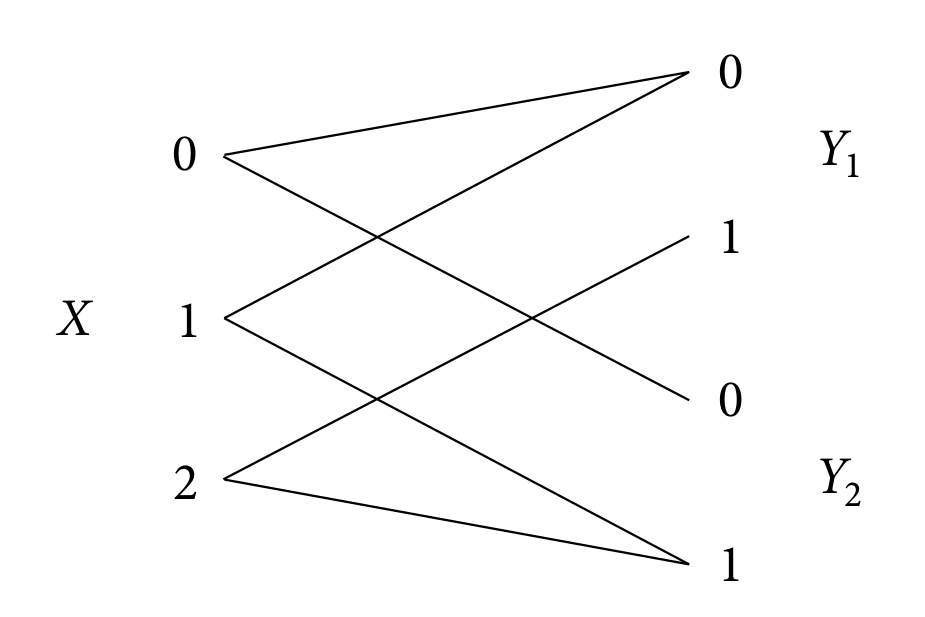
\includegraphics[scale=0.3]{Blackwell.png}
    \caption{The Blackwell channel \cite{Meulen75}}
  \end{center}
\end{figure}

Its capacity region is known (deterministic broadcast channel):

\begin{figure}[!h]
  \begin{center}
    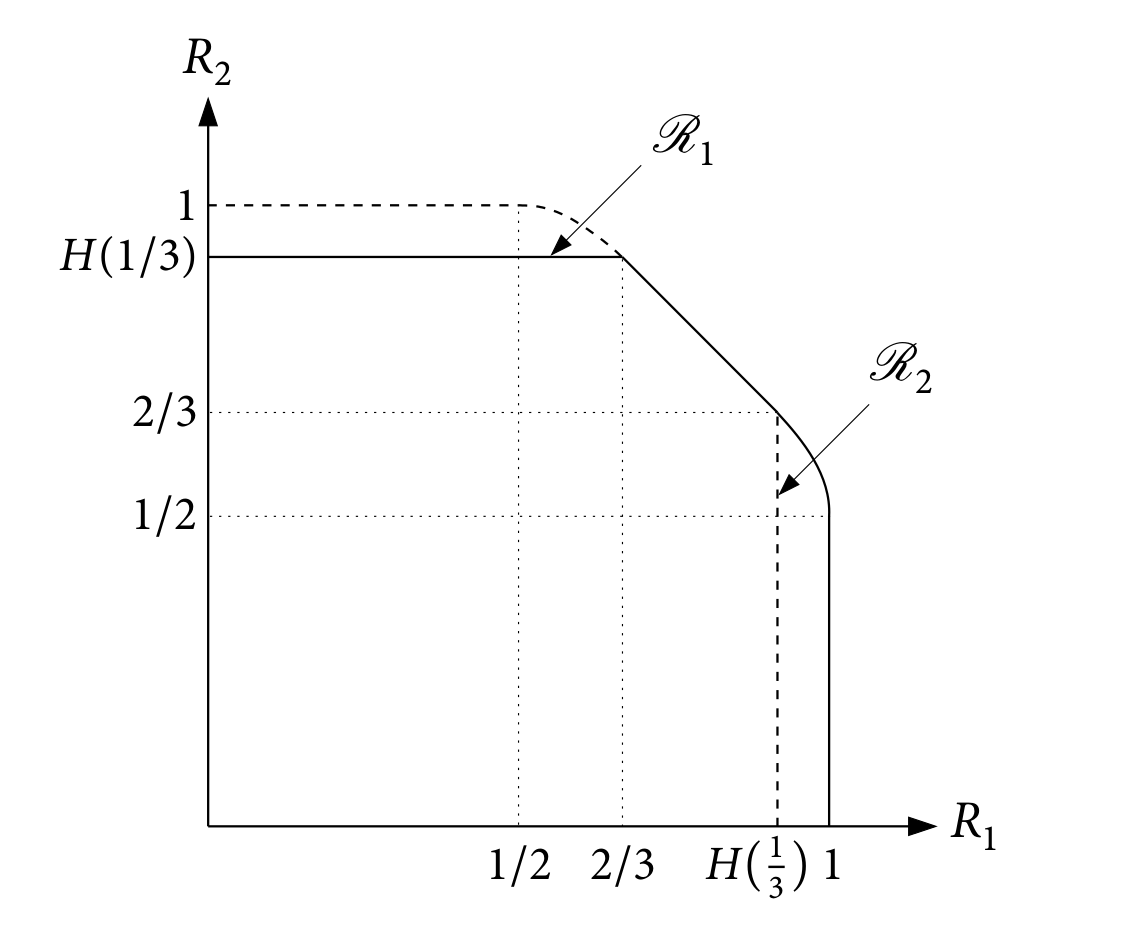
\includegraphics[scale=0.4]{BlackellRateRegion.png}
    \caption{Blackell channel's capacity region}
  \end{center}
\end{figure}

We have then $W_1(0)=W_1(1)=0, W_1(2)=1$ and $W_2(0)=0, W_2(1)=W_2(2)=1$.

%%%   BIBLIOGRAPHY   %%%
\bibliographystyle{plainurl}
\bibliography{Broadcast}
\end{document}
